% Preamble
\documentclass[11pt]{report}

% Packages
\usepackage[a4paper]{geometry}
\usepackage[english]{babel}
\usepackage[backend=biber,style=ieee]{biblatex}
\usepackage{csquotes}
\usepackage[indent=20pt]{parskip}
\usepackage{hyperref}
\usepackage{graphicx}
\usepackage{listings}
\usepackage{subfiles}
\usepackage[table,xcdraw]{xcolor}
\usepackage[normalem]{ulem}
\usepackage{colortbl}
\usepackage{float}
\usepackage{booktabs}
\usepackage{tcolorbox}
\usepackage{aaufrontmatter}

% textidote: ignore begin
\useunder{\uline}{\ul}{}
% textidote: ignore end

% textidote: ignore begin

% Bibliography
\addbibresource{problem-analysis/chess.bib}
\addbibresource{problem-analysis/state-of-the-art/SOTA.bib}
\addbibresource{problem-analysis/target-group-analysis.bib}
\addbibresource{problem-analysis/learning.bib}
\addbibresource{problem-analysis/relevance.bib}
\addbibresource{method/technology.bib}
\addbibresource{problem-solution/software-req-spec.bib}
\addbibresource{problem-solution/backend.bib}
\addbibresource{process-analysis/process-analysis.bib}
\addbibresource{discussion/llm-implementation.bib}

% Configuration
\graphicspath{ {./images/} }

\hypersetup{pdfborder=0 0 0}

% textidote: ignore end

% Document
\title{Conquer the Chessboard}
\subtitle{A Beginner's Journey with AI Coaching}
\theme{Software Engineering}
\semester{Spring}
\groupnumber{8}
\groupmembers{
    Kristiyan Mariyan Georgiev,
    Mads Heilmann,
    Martin Kedmenec,
    Sebastian Hemmer Bech Mygind,
    Simon Woidemann
}
\supervisors{Andres Masegosa}
\department{Software}
\abstract{This project aims to facilitate learning of the game chess by replacing the traditional coach with a
chess engine.
The key focus points of the report are the learning aspect of chess, primarily focusing on why assisted
learning, such as coaching, is more effective than individual learning.
The outcome is an online multiplayer game, where two people can play against each other, while
receiving coaching from the engine in the form of feedback on the players' moves, and suggest improvements.
The project concludes with a discussion on how AI can be used to improve the chess learning experience}
\begin{document}
    % Title
    \maketitle

    % Table of Contents
    % textidote: ignore begin
    \tableofcontents
    % textidote: ignore end

    \makeaaupreface{This is the preface.}

    % Main Content
    % textidote: ignore begin

\lstdefinestyle{pythonStyle}{
    language=Python,
    basicstyle=\ttfamily\small,
    commentstyle=\color{gray},
    keywordstyle=\color{blue},
    stringstyle=\color{green},
    numberstyle=\tiny\color{gray},
    identifierstyle=\color{black},
    backgroundcolor=\color{lightgray!20},
    frame=single,
    frameround=tttt,
    numbers=left,
    numbersep=5pt,
    breaklines=true,
    breakatwhitespace=true,
    tabsize=4,
    showspaces=false,
    showstringspaces=false,
    upquote=true,
    emph={[2]True,False,None},
    emphstyle={[2]\color{purple}},
    emph={[3]range,len},
    emphstyle={[3]\color{orange}},
}

% textidote: ignore end

    % textidote: ignore begin
\chapter{Introduction}\label{ch:introduction}
% textidote: ignore end

Learning is something we do every day.
It is something most people enjoy and strive to experience.
However, learning can also be difficult.
In this report we will explore the concept of collaborated assisted learning and how software can assist in this method.
We will be focusing our analysis around the age-old game of chess.

AI and chess engine popularity has risen greatly in the past years and have been developed to a point that they
outperform humans.
These tools are essential to understanding the complexity of the end- and mid-game strategies of chess.
Chess encapsulates the spirit of a game that is easy to learn, but hard to master.
We will be focusing on the learning part by efficiently and strategically teaching beginners the rules and common
strategies of the game using the capabilities of available chess engines.

    % textidote: ignore begin
\chapter{Problem analysis}\label{ch:problem-analysis}

% textidote: ignore begin
\section{Overview of the problem analysis}\label{sec:overview}

\textbf{Why Play games?}

\begin{itemize}
    \item Social activity.
    \item Fun.
    \begin{itemize}
        \item Although extremely broad every reason for playing a game ultimately leads to enjoyment or fun.
        Many different people enjoy many different games, some physical, some mental,
        but ultimately you play a game to have fun.
        This can be had either through the intricacies of the game itself,
        or because of the social interactions you get while playing games.
    \end{itemize}
\end{itemize}

\textbf{Chess and its genre}

\begin{itemize}
    \item Board game.
    \item Abstract strategy game.
    \item Mind sport.
\end{itemize}

\textbf{Why play chess?}

\begin{itemize}
    \item Playing to win
    \begin{itemize}
        \item When you win a game of chess you have outplayed
        your opponent which creates enjoyment.
        \item Competitive game.
    \end{itemize}
\end{itemize}

\textbf{Who plays chess?}

\begin{itemize}
    \item Non-competitive
    \begin{itemize}
        \item This Group of players enjoy chess as a game casually,
        they might not know all the intricacies of chess.
        \item The experience of this subsection of players range from: Beginner - competent
    \end{itemize}
    \item Competitive
    \begin{itemize}
        \item To play chess competitively you need to have a good understanding
        of the game and the underlying principles of how you win.
        \item The experience of this subsection ranges from competent - master level
    \end{itemize}
\end{itemize}

\textbf{State of the art}

\begin{itemize}
    \item Chess.com
    \begin{itemize}
        \item Play chess
        \begin{itemize}
            \item Different time modes
            \item different variations like, 4 player chess
            \item Tournaments
        \end{itemize}
        \item Learn chess
        \begin{itemize}
            \item Puzzles
            \item Playstyles
            \item Theory, openings and endgames.
            \item Analyze a game of chess using engines
        \end{itemize}
        \item Coaching
    \end{itemize}
    \item Lichess.org
    \begin{itemize}
        \item Although both Lichess.org and Chess.com are free in the beginning,
        chess.com limits functionality to sell a premium service,
        this is opposed to Lichess.org which is complete free,
        both in terms of cost, but the website is also open-source.
        \begin{itemize}
            \item You can also play chess and different variations on Lichess
            \item Lichess has a more comprehensive learning section.
            \item Coaching
        \end{itemize}
    \end{itemize}
\end{itemize}

\textbf{Weaknesses in the state of the art}

\begin{itemize}
    \item As mentioned above, when learning chess you have ample opportunity for learning through puzzles analysis,
    but what all these things have in common, or lack is “human contact”.
    When learning chess the only viable options are studying or learning with a computer.
    This leaves an opening in finding some way to incorporate learning chess specifically while playing with someone
    else and having the social aspect that is more characteristic of non-competitive chess.
\end{itemize}

\textbf{Target audience}

\begin{itemize}
    \item The product mentioned above would be some way to learn chess
    while playing with someone else that has a learning aspect incorporated into the chess game beyond simply playing.
    \begin{itemize}
        \item As you will receive help this is not a website build for competitive use.
        \item The implementation could be allowing some level of engine help while playing, and because chess
        engines are at a level far beyond human capabilities, the ceiling for learning through this method is unclear.
    \end{itemize}
\end{itemize}
% textidote: ignore end

% textidote: ignore end

% textidote: ignore begin
\section{Chess}\label{sec:chess}
% textidote: ignore end

Chess is a game that has existed for millennia.
It has roots in India as well as China where the first iterations of chess we know today was invented~\cite{murray1913}.

Nowadays, the chess standard universally known as chess is the iteration of the game called international chess or
western chess, which is also the standard that FIDE, the international chess governing body, uses~\cite{fide2024}.

Most people are familiar with chess, hereby the rules of the game and the look of the board.
We will therefore only mention a few key elements of chess and online chess, which are not as common knowledge and will
be important for understanding the technicalities of chess.

\subsection{Notation}\label{subsec:notation}

Notation in chess regards how one is able to communicate the events of a particular game in writing.
The modern standard is the algebraic notation, where the rows are named from `1' through `8' going from white to black
and the columns are named from `a' through `h' going from queen-side to king-side.
As an example, the notation `a1' refers to the bottom left cell from white's perspective~\cite{pickel2022}.

As seen in Figure~\ref{fig:chess-notation-example}, when moving, one specifies the piece to be moved and the
destination.
In the line labeled `1' only the destination is mentioned in both moves, which implies that it was pawn moves.
In the line labeled `4' there is an `x' implying the capture of another piece as a result of the move.

% textidote: ignore begin
\begin{figure}[h]
    \centering
    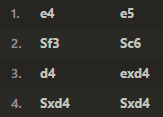
\includegraphics[width=0.5\textwidth]{chess-notation-example}
    \caption{Chess notation example~\cite{chess.com2024}}.\label{fig:chess-notation-example}
\end{figure}
% textidote: ignore end

This notation style is efficient and is also the way computers write and read moves.
The \lstinline{pgn} file extension is used for text files that encapsulates completed chess games.
Only one game is stored per file~\cite{chess.com2024}.

% textidote: ignore begin

\subsection{Rules}\label{subsec:rules}
% textidote: ignore end

Another important aspect of the game of chess is the more complicated rules.
These are desirable to implement into any chess game.
Below a few of the important more scarcely known rules are mentioned:

\begin{itemize}
    \item \textbf{Time control}: Different tournaments and types of games have different time control rules, such as
    rewarding time after every move.
    Another example is the game type Armageddon, where black and white have different starting times on the
    clock~\cite{schiller2012}.
    \item \textbf{Draw}: Drawing or tying in chess can happen in different ways.
    Examples include stalemate, the 50 move rule and repetition~\cite{schiller2012}.
    \item \textbf{En passant}: A pawn can capture another pawn, if the second mentioned pawn was moved by a double move
    to either adjacent side of the first mentioned pawn~\cite{schiller2012}.
\end{itemize}

These rules as well as all other rules will need to be implemented into any chess game for it to have the same features
as standard over-the-board chess.

% textidote: ignore begin
\section{Learning}\label{sec:learning}
% textidote: ignore end

The group comprises five of the students from the P1 project.
Therefore, the students in the group are familiar with each other, both on a personal and an academic level.
As per P1, the P2 project tech-stack is rather complicated and out of scope.
However, as the group is very ambitious and wants to learn relevant technologies, this complexity is welcomed.

Some technologies the group learned throughout the project are:

\begin{itemize}
    \item \textbf{Docker}: Docker is vital for the development environment for all the members of the group, as all the
    three main operating systems, Windows, macOS and Linux, are represented in the group.
    Learning this tool made for a smoother development process and probably for significantly less time debugging.
    \item \textbf{TypeScript}: As JavaScript is a rather complicated programming language that has a lot of weird
    behavior, especially from the eyes of beginners, the group learned TypeScript, as it provided better and more
    type safe code.
    \item \textbf{React}: As HTML, CSS and JavaScript is a rather bare-bones, it takes a lot of time to code beautifully
    and efficiently using just these technologies, why React had to be learned.
    React made for more efficient development and for better readability, which helped the group better communicate
    about the code and better understand the code others have written.
    % textidote: ignore begin % due to next.js being identified as an url
    \item \textbf{Next.js}: Next.js provided the group with an easier way of routing by using the file system using the
    app directory among other useful features.
    % textidote: ignore end
    This framework once again made for more efficient code writing and understandability that the group benefited
    greatly from.
    \item \textbf{Python}: For the parsing of the Stockfish executable output a Python script was used, why the group
    had to learn the foundational elements of the Python programming language.
    Learning this technology was necessary for the project and will also most probably help the group members in their
    later career, why it was decided to learn it.
\end{itemize}


\section{Multiplayer}\label{sec:multiplayer-analysis}

Chess is famously played by two players, where each player takes turns to move their pieces.
Because of this, the game is inherently a multiplayer game.
There are however different types of multiplayer games, and while chess is originally a tabletop game, adapting it to a
digital platform has an effect on the multiplayer aspect of the game.
This section will go over the different types of multiplayer games, and how the transition from local to online
multiplayer can have an effect on learning chess.

\subsection{Types of multiplayer games}\label{subsec:types-of-multiplayer-games}

Multiplayer is a term used to describe games that can be played by more than one player.
It is mostly associated with video games, but most tabletop games, such as chess, are also multiplayer games.
Throughout the years, there have been three dominating types of multiplayer implementations~\cite{multiplayer-types},
and chess can fall into two of these types.

\begin{itemize}

    \item \textbf{Local multiplayer} has the players take turns to play the game.
    It requires the players to be in the same room and to wait for their turn to play.
    Traditional tabletop games, such as chess, fall into this category.

    \item \textbf{Co-op multiplayer} has two players playing on a split-screen.
    It also requires the players to be in the same room, but unlike the first type, they can play at the same time.
    This type is mostly associated with video games, and it is not relevant for chess.

    \item \textbf{Online multiplayer} allows for players to play together over the internet, negating the requirement to
    be in the same room as with the previous two types.
    This type of multiplayer can be seen in online chess games.

\end{itemize}

It can be concluded that by adapting chess to a digital platform, its multiplayer changes from local to online
multiplayer.
While the game itself remains the same, the way players interact with each other changes drastically.
This can have an impact on the experience players have when learning and playing chess.

\subsection{Effects multiplayer has on learning}\label{subsec:effects-multiplayer-has-on-learning}

Online multiplayer has a lot of benefits over local multiplayer.
It makes it possible to connect with people from all over the world, as they don't have to be in the same room.
It also allows for people to play against strangers, usually in a competitive environment, fitting for chess.
However, it takes away from the social aspect of the game, as players rarely communicate with each other.

There are different arguments on the matter, one source praises how online multiplayer allows for people to connect and
socialize with people they never could before~\cite{multiplayer-online}, while another source complains about how
transitioning from local to online multiplayer has significantly impacted the social interaction with their
friend~\cite{multiplayer-local}.
Online multiplayer games often attempt to mitigate the lack of social interaction by implementing chat, voice or video
systems, but it is rare for players, especially strangers, to use these features.

This lack of communication can have a negative effect on learning chess, as it discourages players from reaching out
for help or advice.
That typically results in a poor experience for novices.
A lot of people would rather learn chess from friends, family or a coach, resulting in a local multiplayer environment.
Therefore, we can conclude that the transition from local to online multiplayer has a negative effect on the learning
experience of chess.


    % textidote: ignore begin
\chapter{Problem statement}\label{ch:problem-statement}
% textidote: ignore end

% textidote: ignore begin
\section{Problem delineation}\label{sec:problem-delineation}
% textidote: ignore end

% textidote: ignore begin
\section{Problem statement}\label{sec:problem-statement}
% textidote: ignore end

How can we make an online multiplayer chess game for beginner players that facilitates learning chess using supervised
learning methods?

    % textidote: ignore begin
\chapter{Method}\label{ch:method}
% textidote: ignore end

\section{Technology}\label{sec:technology}

Throughout the development of the project, a number of different tools and publicly available packages are used to
assist the development process.
These different technologies were chosen based on the team's needs and the requirements of the project.
The following sections will describe the different technologies used in the project.

\subsection{Programming stack}\label{subsec:programming}

As the project is a web application, TypeScript~\cite{typescript} is used as the main programming language.
TypeScript is a superset of JavaScript, with the main difference being that TypeScript is statically typed, while
JavaScript is dynamically typed.
It can be very useful in larger projects, as it helps to catch errors during compile-time as opposed to run-time.
This is the first time for many of the team members to use TypeScript, but they find it to be safer than JavaScript
for larger projects.

The frontend of the project is built with React~\cite{react}, which is a JavaScript/TypeScript library for building
user interfaces.
It is developed and maintained by Meta, and is used by many large companies.
React is focused on mobile applications first and foremost, however it is also useful for desktop applications, why it
is chosen as the top level UI library.

% textidote: ignore begin % due to node.js and next.js being identified as an url
The backend is built using Node.js~\cite{node.js}, which allows the team to build server-side components using
TypeScript.
Node.js is a popular choice for backend development, as it is fast and scalable.
As well as using React for client-side rendering, Next.js~\cite{next.js} is incorporated to handle the server-side
rendering.
Next.js is a React framework running on top of Node.js, which assists in building the frontend and backend
together.
% textidote: ignore end

\subsection{JavaScript libraries}\label{subsec:libraries}

Throughout the project the team uses a number of different libraries to aid with the mundane tasks of web development.
% textidote: ignore begin % Due to chess.js being identified as an url
For example, as the focus was on the learning aspect of the project, the team uses Chess.js~\cite{chess.js} to handle
the chess logic and react-chessboard~\cite{react-chessboard} to display the chessboard.
% textidote: ignore end
This saves a lot of time, as chess is a complex game with many rules.

The team also uses Material UI~\cite{mui} (MUI) to style the website, as it is a modern and popular library that
uses Google's design language, Material Design.
MUI is used to create the buttons, text fields, and other components that make up the website.

Lastly, the team uses Chatscope~\cite{chatscope} to create the chat window of the website.
The chat window is an important element of the website, as it allows users to communicate with Stockfish or with each
other.

% textidote: ignore begin
\subsection{Hosting provider}\label{subsec:hosting}
% textidote: ignore end

There are a number of different hosting providers available.
Amazon Web Services~\cite{aws} is a popular choice, but it can be expensive.
Instead, Firebase~\cite{firebase} is chosen due to its features and pricing.
The main reason for this decision is that Firebase allows for easy authentication with Google accounts, which was
essential for building the lobby system.

% textidote: ignore begin % Due to socket.io being identified as an url
Socket.io~\cite{socket.io} was considered for the multiplayer aspect, but it can't be used with Firebase.
% textidote: ignore end
However, Firebase provides a real-time database, which was extensively used throughout the project instead.
The real-time database works like a normal database, but with the added benefit of being able to listen for changes in
real time and having very little delay between the data being sent and received.
% textidote: ignore begin % Due to socket.io being identified as an url
It was used as a replacement for Socket.io, as the latency was low enough for the team's needs.
% textidote: ignore end
The database saves game states, chat messages, lobbies and other data.

% textidote: ignore begin
\section{Development process}\label{sec:development-process}
% textidote: ignore end

This section describes the different elements of the development process.
Other development processes and protocols exist in the team; however, only the most important ones are mentioned in the
following sections.

% textidote: ignore begin

\subsection{Development environment}\label{subsec:development-environment}
% textidote: ignore end

The project requires a number of different services to be running at the same time, which can be challenging to manage.
% textidote: ignore begin % Due to node.js being identified as an url
That is the Node.js backend, Stockfish and Firebase Emulator.
% textidote: ignore end
To manage them, the team uses Docker~\cite{docker} to simultaneously run all the services.
Docker is a platform that allows developers to isolate their applications in containers, which are lightweight and can
run on any machine on any operating system.
This makes it painless to develop multiservice projects, as there are no compatibility issues between the different
devices and services.
To handle multiple containers, the team uses Docker Compose, which is a tool for defining and running multi-container
Docker applications.
This makes it possible to run all the services locally when developing, simulating how they will behave in a production
environment.

% textidote: ignore begin

\subsection{CI/CD}\label{subsec:ci/cd}
% textidote: ignore end

The team uses GitHub~\cite{github} for version control and continued integration and development (CI/CD) for both the
report writing process and the development of the software.
GitHub provides many features, such as Pull Requests, Issues, Actions, and Projects, which makes it easy to collaborate
and work on the project and the report.

The team uses branches, where the unwritten rules is that only the creator of the branch makes changes to the code in
the branch to avoid accidental overwriting of code.
Having branches makes it simple to track what team members are working on and how far in development they are.

\subsubsection{Task management}

The team makes use of GitHub projects to plan out different tasks and issues to track bugs and features.
A snapshot of some categories with some issues can be seen in Figure~\ref{fig:github-project}.
In the figure, it is clear that issues move from category to category as the team progresses with them.

The custom protocol is for a team member to assign one self to an issue and thereafter complete the task associated with
the issue.
This way, other team members can comment inside the issue if they have comments about what the issue entails.
Another reason for this method is that it is clear to all members what problems are being solved in a given pull request
as the relevant issue is linked, thereby improving efficiency and clarity.
This method of creating issue and assigning one self to them makes for a lot of freedom in development.

This freedom, however, comes with the responsibility for team members to adequately assign themselves to enough issues
to cover their respective workload commitments.
Having the list of issues dynamically update, as team members resolve them, makes for a clean and
comprehensible overview of how much work needs to be done, how much is in progress, and how much has been done.

% textidote: ignore begin
\begin{figure}[htb]
    \centering
    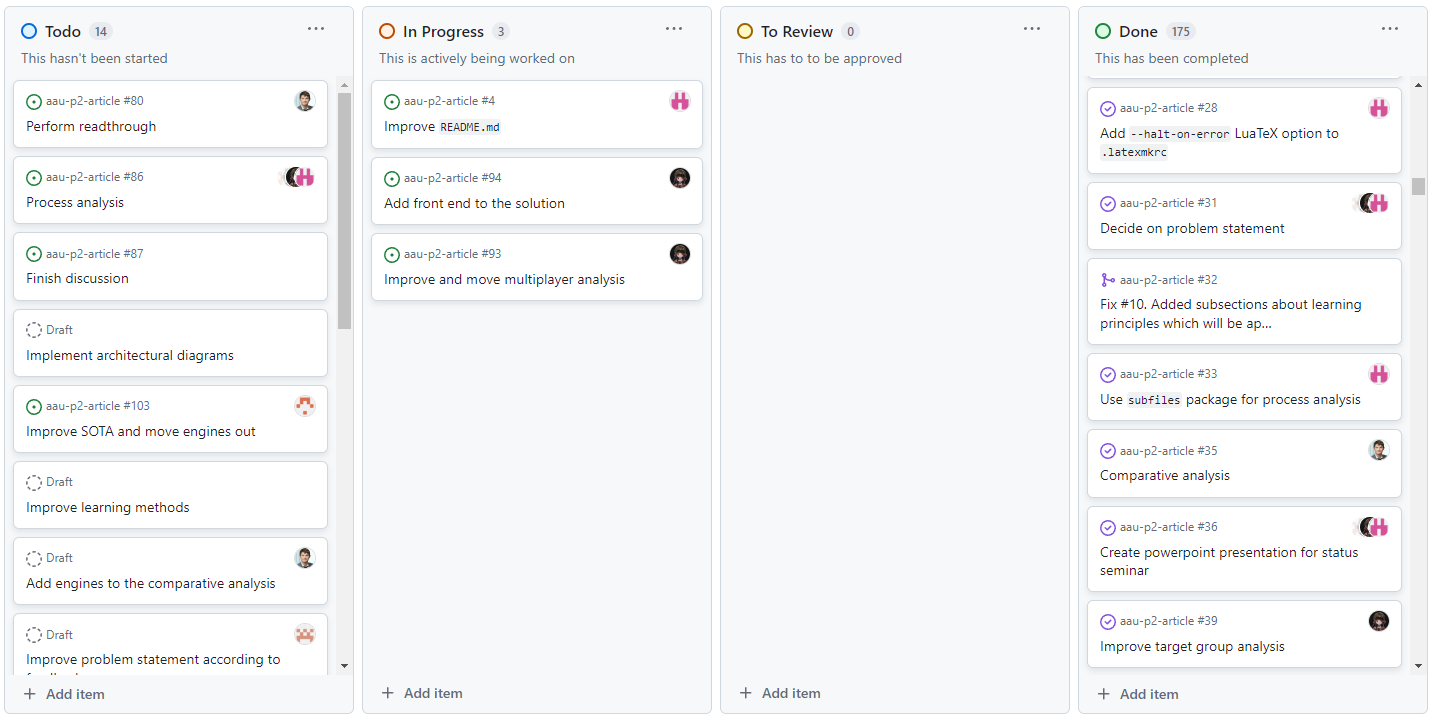
\includegraphics[width=1\textwidth]{github-projects}
    \caption{GitHub Project overview.}\label{fig:github-project}
\end{figure}
% textidote: ignore end

% textidote: ignore begin

\subsubsection{Automation}
% textidote: ignore end

GitHub Actions are used to run custom checks among others automatically.
Having the actions run on all lines of code makes for the security that other team members code is living up to the
standards desired and agreed on by the team.
Different actions are relevant for the four different repositories that make up the entire project codebase.
Reference to the repositories is made to Appendix~\ref{ch:source-code-repositories}.
The two repositories with the most changes throughout the development process are those for the report and the
front-end.
The focus is therefore on the actions for these, even though the other repositories also have GitHub Actions
attached to them.
In Table~\ref{tab:actions-overview} it can be seen that the team mainly uses five different actions.
In the table is also provided the main purpose of the action and a small description of them.
These actions make for more efficient, more understandable and more reliable code, why they are used.

% textidote: ignore begin
\begin{table}[h]
    \centering
    \resizebox{\columnwidth}{!}{%
        \begin{tabular}{clllll}
            \toprule
            \rowcolor[HTML]{9B9B9B}
            \textbf{Actions} & \multicolumn{2}{c}{\cellcolor[HTML]{9B9B9B}\textbf{Attributes}} \\ \midrule
            \rowcolor[HTML]{EFEFEF}
            \cellcolor[HTML]{C0C0C0}{\color[HTML]{000000} \textit{\textbf{Report}}}    &
            \multicolumn{1}{c}{\cellcolor[HTML]{EFEFEF}\textbf{Purpose}}  &
            \multicolumn{1}{c}{\cellcolor[HTML]{EFEFEF}\textbf{Description}}
            \\ \midrule
            \cellcolor[HTML]{EFEFEF}\textbf{xu-cheng's latex-action}                   & \begin{tabular}[c]{l}
                                                                                             Compiles the latex document
            \end{tabular} & \multicolumn{1}{l}{\begin{tabular}[c]{l}
                                                   This action is made by a private person and runs \\
                                                   a docker container with TexLive installed
            \end{tabular}}                                 \\ \midrule
            \cellcolor[HTML]{EFEFEF}\textbf{TeXtidote}                                   & \begin{tabular}[c]{l}
                                                                                               Lints the latex document
            \end{tabular} & \multicolumn{1}{l}{\begin{tabular}[c]{l}
                                                   This action utilizes the TeXtidote binary to lint \\
                                                   the report for any spelling mistakes
            \end{tabular}} \\ \midrule
            \cellcolor[HTML]{EFEFEF}\textbf{Chk TeX}                                    & \begin{tabular}[c]{l}
                                                                                              Formats the latex document
            \end{tabular} & \multicolumn{1}{l}{\begin{tabular}[c]{l}
                                                   This action makes use of Chk TeX, which checks for \\
                                                   common mistakes in latex.
                                                   The group mostly uses \\
                                                   it to format tables and images correctly
            \end{tabular}}                                  \\ \midrule
            \rowcolor[HTML]{EFEFEF}
            \cellcolor[HTML]{C0C0C0}{\color[HTML]{333333} \textit{\textbf{Front-end}}}
            & \multicolumn{1}{c}{\cellcolor[HTML]{EFEFEF}\textbf{Purpose}}        &
            \multicolumn{1}{c}{\cellcolor[HTML]{EFEFEF}\textbf{Description}}     \\ \midrule
            \cellcolor[HTML]{EFEFEF}\textbf{ESLint}                                  & \begin{tabular}[c]{l}
                                                                                           Lints the software
            \end{tabular}        & \multicolumn{1}{l}{\begin{tabular}[c]{l}
                                                          ESLint is used mostly for the best practise \\
                                                          comments it provides, such that the group follows \\
                                                          the same guidelines when coding
            \end{tabular}}                                  \\ \midrule
            \cellcolor[HTML]{EFEFEF}\textbf{Prettier}                                  & \begin{tabular}[c]{l}
                                                                                             Formats the software
            \end{tabular}        & \multicolumn{1}{l}{\begin{tabular}[c]{l}
                                                          Prettier makes sure that the code is indented \\
                                                          correctly among other formatting settings
            \end{tabular}}                                  \\ \bottomrule
        \end{tabular}%
    }
    \caption{Overview of the most used actions for the report and the software.}\label{tab:actions-overview}
\end{table}
% textidote: ignore end

% textidote: ignore begin

\subsubsection{Quality control}
% textidote: ignore end

Another important process mechanism the team uses is the pull request feature of GitHub.
In the pull request is where changes to be merged into the main branch are displayed as well as where the GitHub Actions
runs are documented.
The custom protocol is for at least two team members to accept the changes made before the commits in the pull request
can be merged into the main branch.
This safety feature makes it such that at least three of the five team members agree with the changes made.
By having this barrier, it also makes sure that individual small changes can also be agreed on, and that they don't get
lost or go unseen by the rest of the team.

One of the advantages to using this method over software like Overleaf is that GitHub provides a log of all changes made
as well as ´blame'.
This makes it possible to see who made the changes at all times in local IDEs.
Being able to quickly identify the author of a line makes communication in the team more efficient.
One of the disadvantages is that development typically takes longer, as every change needs to be reviewed by the team
before being able to be merged.


    % textidote: ignore begin
\chapter{Problem solution}\label{ch:problem-solution}
% textidote: ignore end

Figure~\ref{fig:software-architecture} provides an overview of the top-level components of the software architecture.
In the following sections we will analyze the choices made in the development of the software and highlight key areas of
the codebase.

% textidote: ignore begin
\begin{figure}[h]
    \centering
    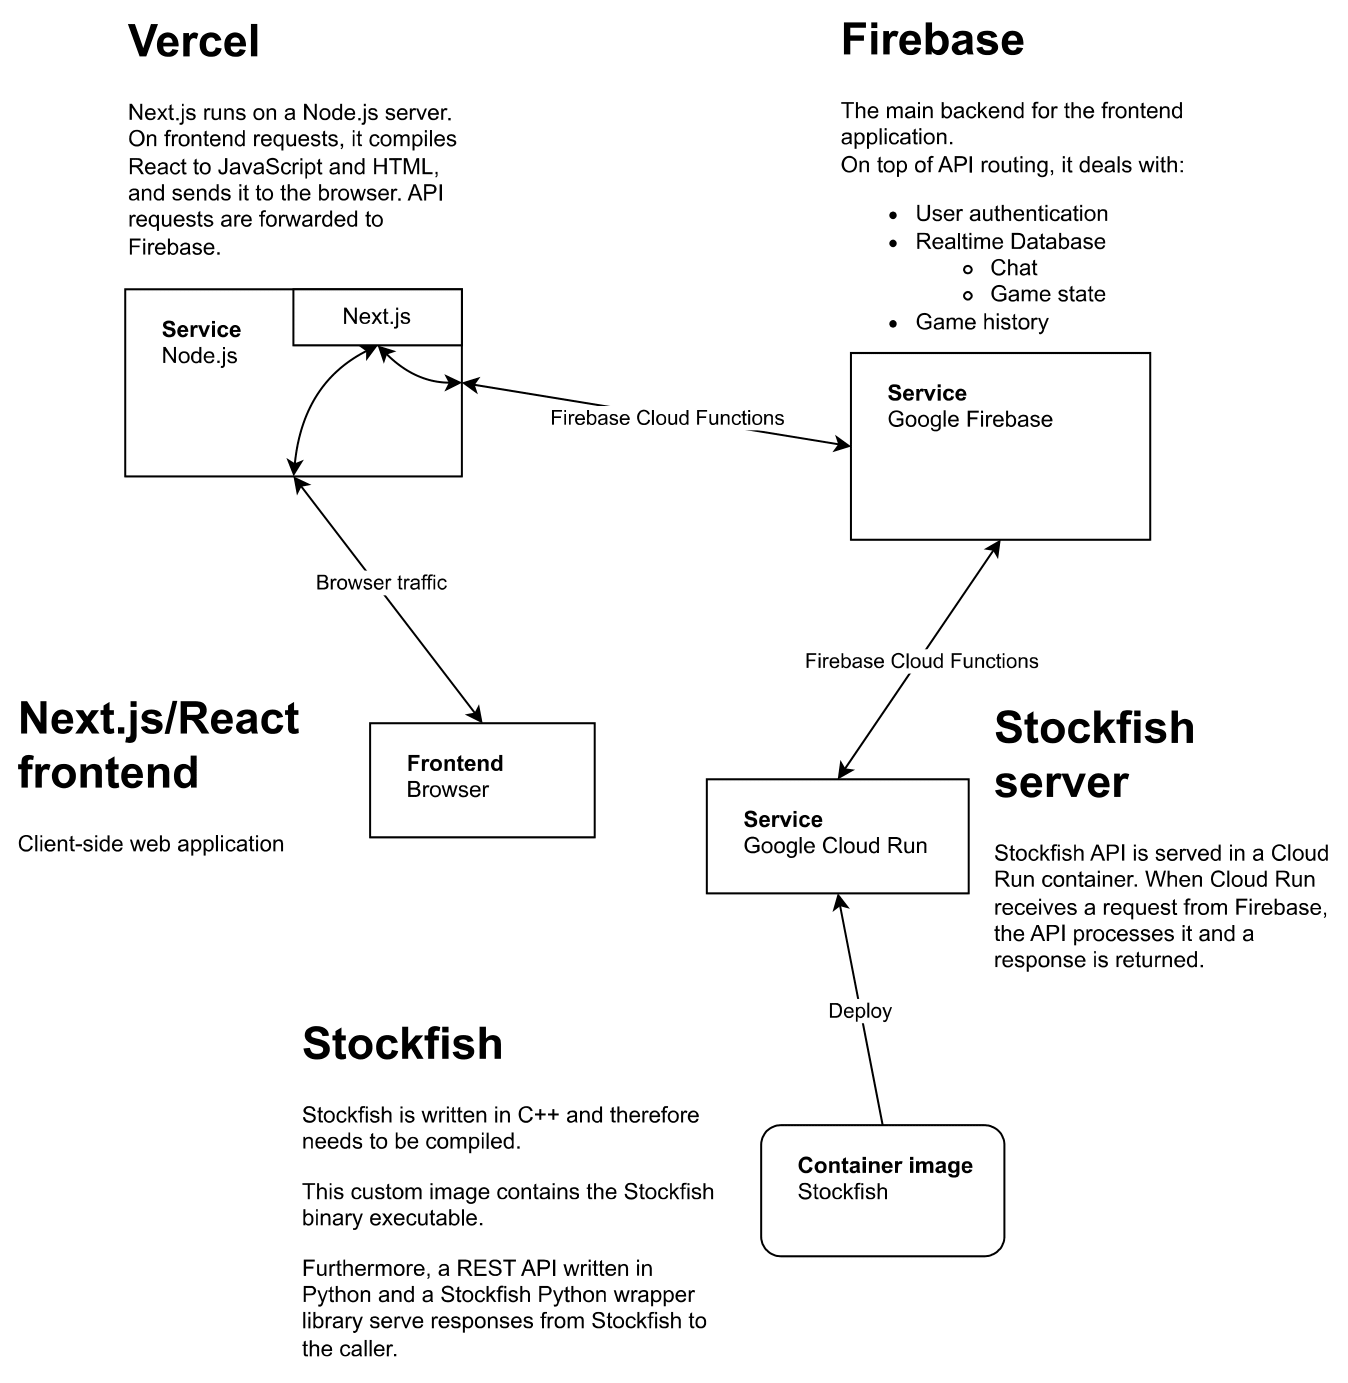
\includegraphics[width=1\textwidth]{architecture}
    \caption{Overview of the architecture of the program.}\label{fig:software-architecture}
\end{figure}
% textidote: ignore end

% textidote: ignore begin
\section{Software requirement specification}\label{sec:software-requirement-specification}
% textidote: ignore end

% textidote: ignore begin
\subsection{Must-haves (Mo)}\label{subsec:must-haves}

\begin{itemize}
    \item Multiplayer functionality
    \item Applied learning principles
    \item Chess engine assistance
\end{itemize}

\subsection{Should-haves (S)}\label{subsec:should-haves}

\begin{itemize}
    \item Tailored engine feedback
\end{itemize}

\subsection{Could-haves (Co)}\label{subsec:could-haves}

\begin{itemize}
    \item XXX
\end{itemize}

\subsection{Won't-haves (W)}\label{subsec:wont-haves}

\begin{itemize}
    \item XXX
\end{itemize}
% textidote: ignore end

% textidote: ignore begin
\section{Front end}\label{sec:frontend}
% textidote: ignore end

The following section is a showcase of the look and feel of the finished product.
It will go over every aspect of the website, from the landing page to the game interface, with explanations on how to
navigate between the pages and arguments for the design choices made.
This serves to inform the reader about the user experience of the website without actually having to visit it.

Upon opening the website, the user is greeted with a landing page, as seen in Figure~\ref{fig:home}.
The landing page serves as a brief introduction to the project, informing the user about the project's goal and purpose.
That page is only visible to users who are not logged in because it's something that the user only needs to see once,
similar to different websites, such as GitHub.
The user can then choose to learn more about the project by clicking on the buttons as seen in
Figure~\ref{fig:home-info}.

% textidote: ignore begin % due to sh:capperiod despite the period being correct
\begin{figure}[H]
    \centering
    \setlength{\fboxsep}{0pt}
    \fbox{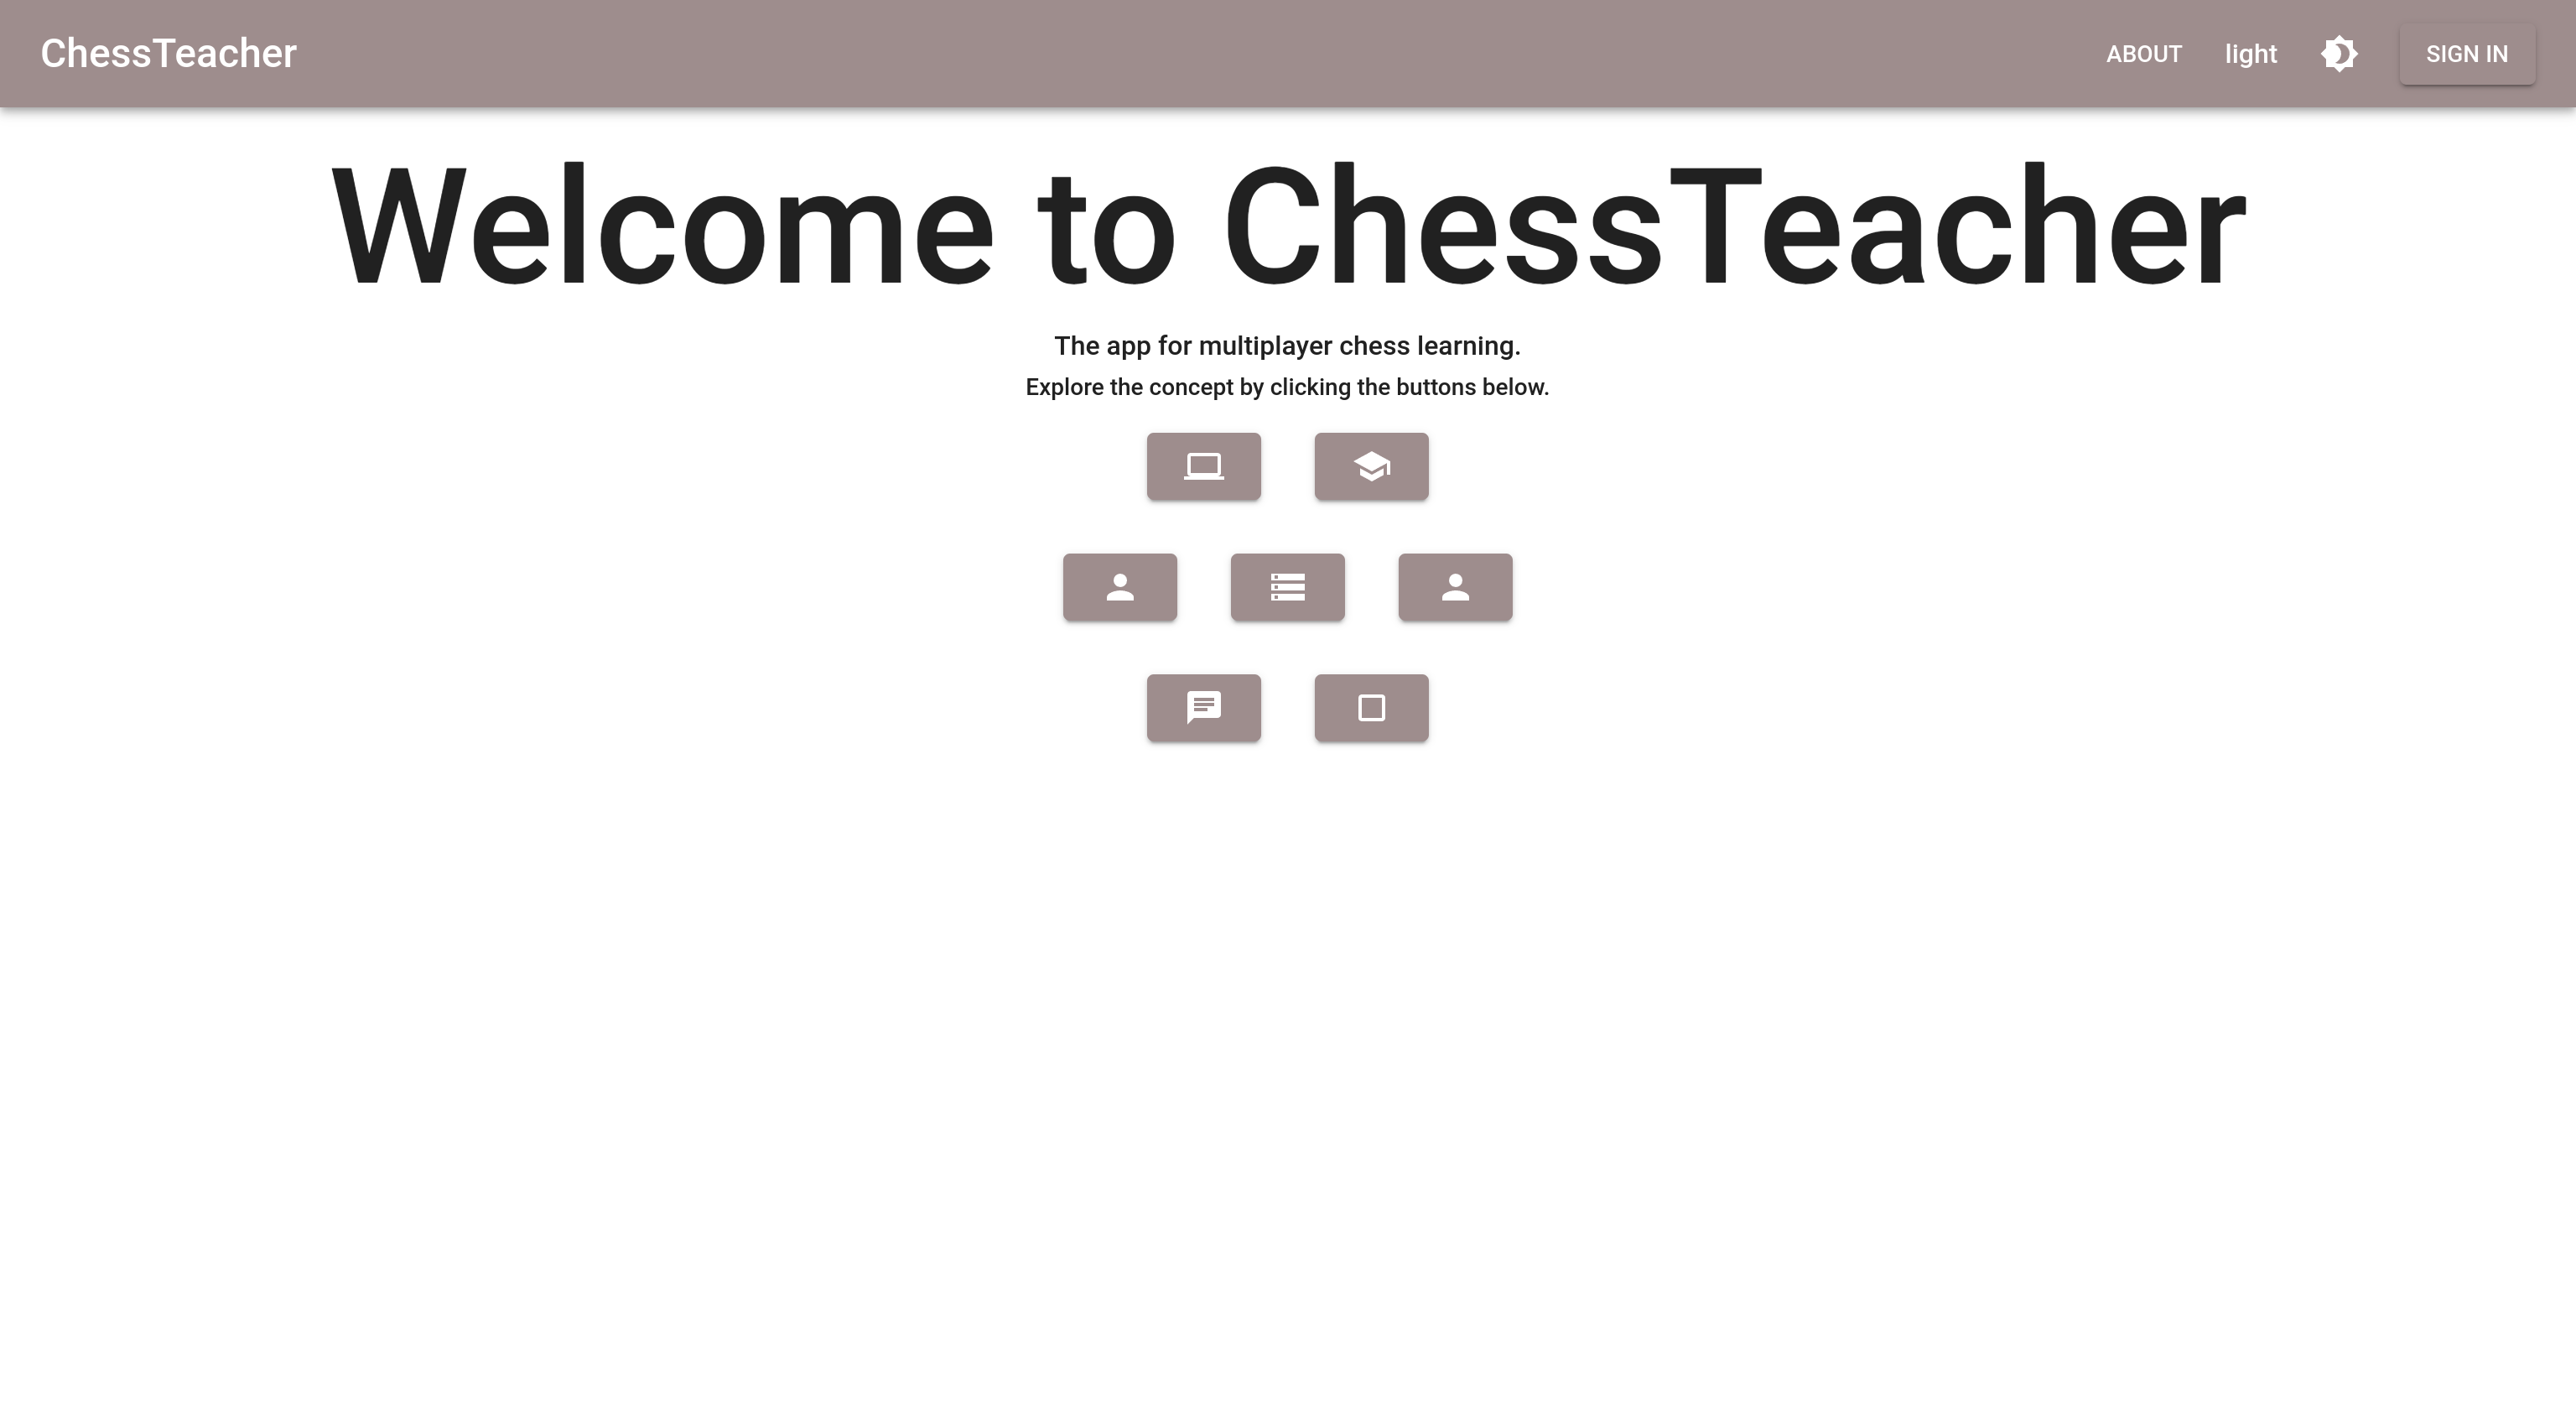
\includegraphics[width=1\textwidth]{frontend-home}}
    \caption{The landing page of the website.}\label{fig:home}
\end{figure}

\begin{figure}[H]
    \centering
    \setlength{\fboxsep}{0pt}
    \fbox{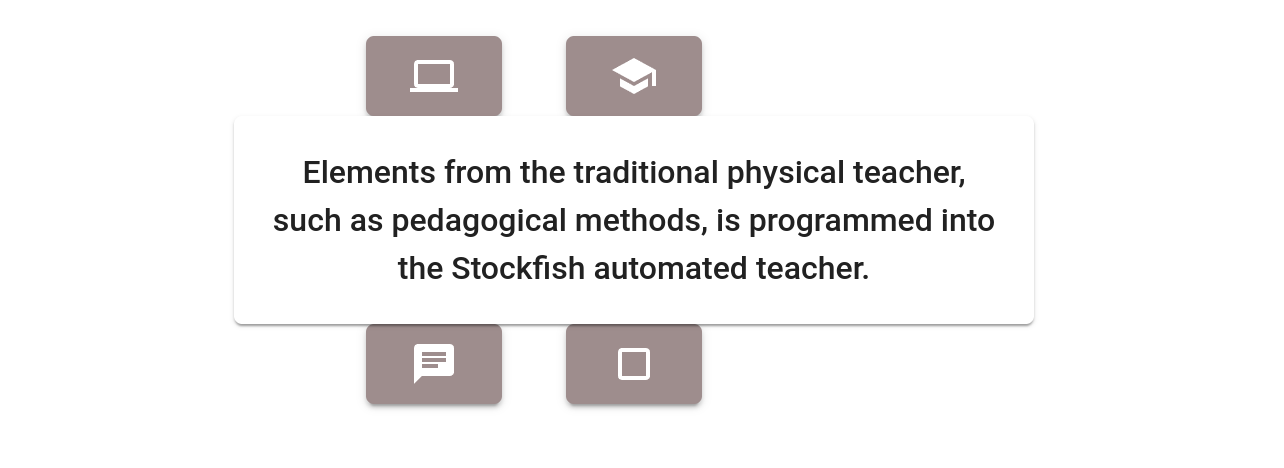
\includegraphics[width=1\textwidth]{frontend-home-info}}
    \caption{More info upon clicking on the buttons.}\label{fig:home-info}
\end{figure}
% textidote: ignore end

To access the game lobby, the user first has to log in.
The login system is based on Firebase Authentication, which was selected for its easy and secure login process.
The user can use their existing Google account to log in, which negates the need for creating a new account.
This makes the login process quick and easy.
To log in, the user has to click on the ``Sign in'' button in the top right corner of the website.
The log in screen can be seen in Figure~\ref{fig:login}.

% textidote: ignore begin
\begin{figure}[H]
    \centering
    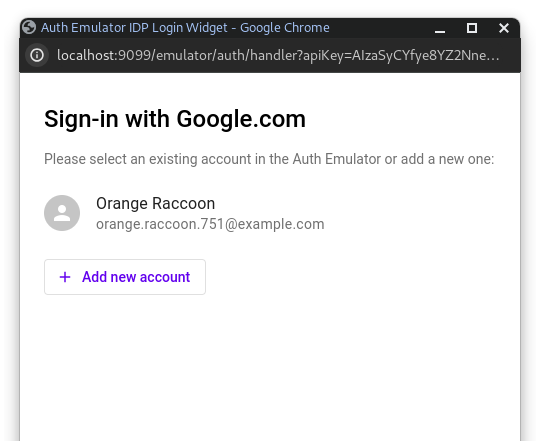
\includegraphics[width=0.8\textwidth]{frontend-login}
    \caption{Google Authentication prompt when logging in.}\label{fig:login}
\end{figure}
% textidote: ignore end

Once the user is authenticated, the home page would lead to the lobby listing, rather than the landing page.
The lobby listing is a list of all the available games that the user can join.
As more users join the website, the lobby listing will be populated with more games, but during development, the lobby
listing is empty, as seen in Figure~\ref{fig:lobby-empty}.

Anyone can create a new game by clicking on the green ``Create New Match'' button in the top right corner of the
listings.
This will create a new entry to the lobby, as seen in Figure~\ref{fig:lobby-game}.
Once a game is created, a different user can join the game by clicking on the green ``Join'' button in the game's entry.
The creator will get a notification, which can be seen in Figure~\ref{fig:lobby-join}.
It will appear in the bottom right corner of the screen, and it serves to inform the creator that someone has joined
their game and that the game can now start.
The notification was added to improve the user experience, as the creator would have no other way of knowing that
someone has joined.
Both players will have to open the game by clicking on the ``View'' button, which will replace the ``Join'' button once
the second player has joined.
Other players can spectate the game by clicking that same button.
The team wanted to add a spectating option to the game, because it would allow for a better learning experience, as
spectators can support the players similar to how the chess engine does.

% textidote: ignore begin
\begin{figure}[H]
    \centering
    \setlength{\fboxsep}{0pt}
    \fbox{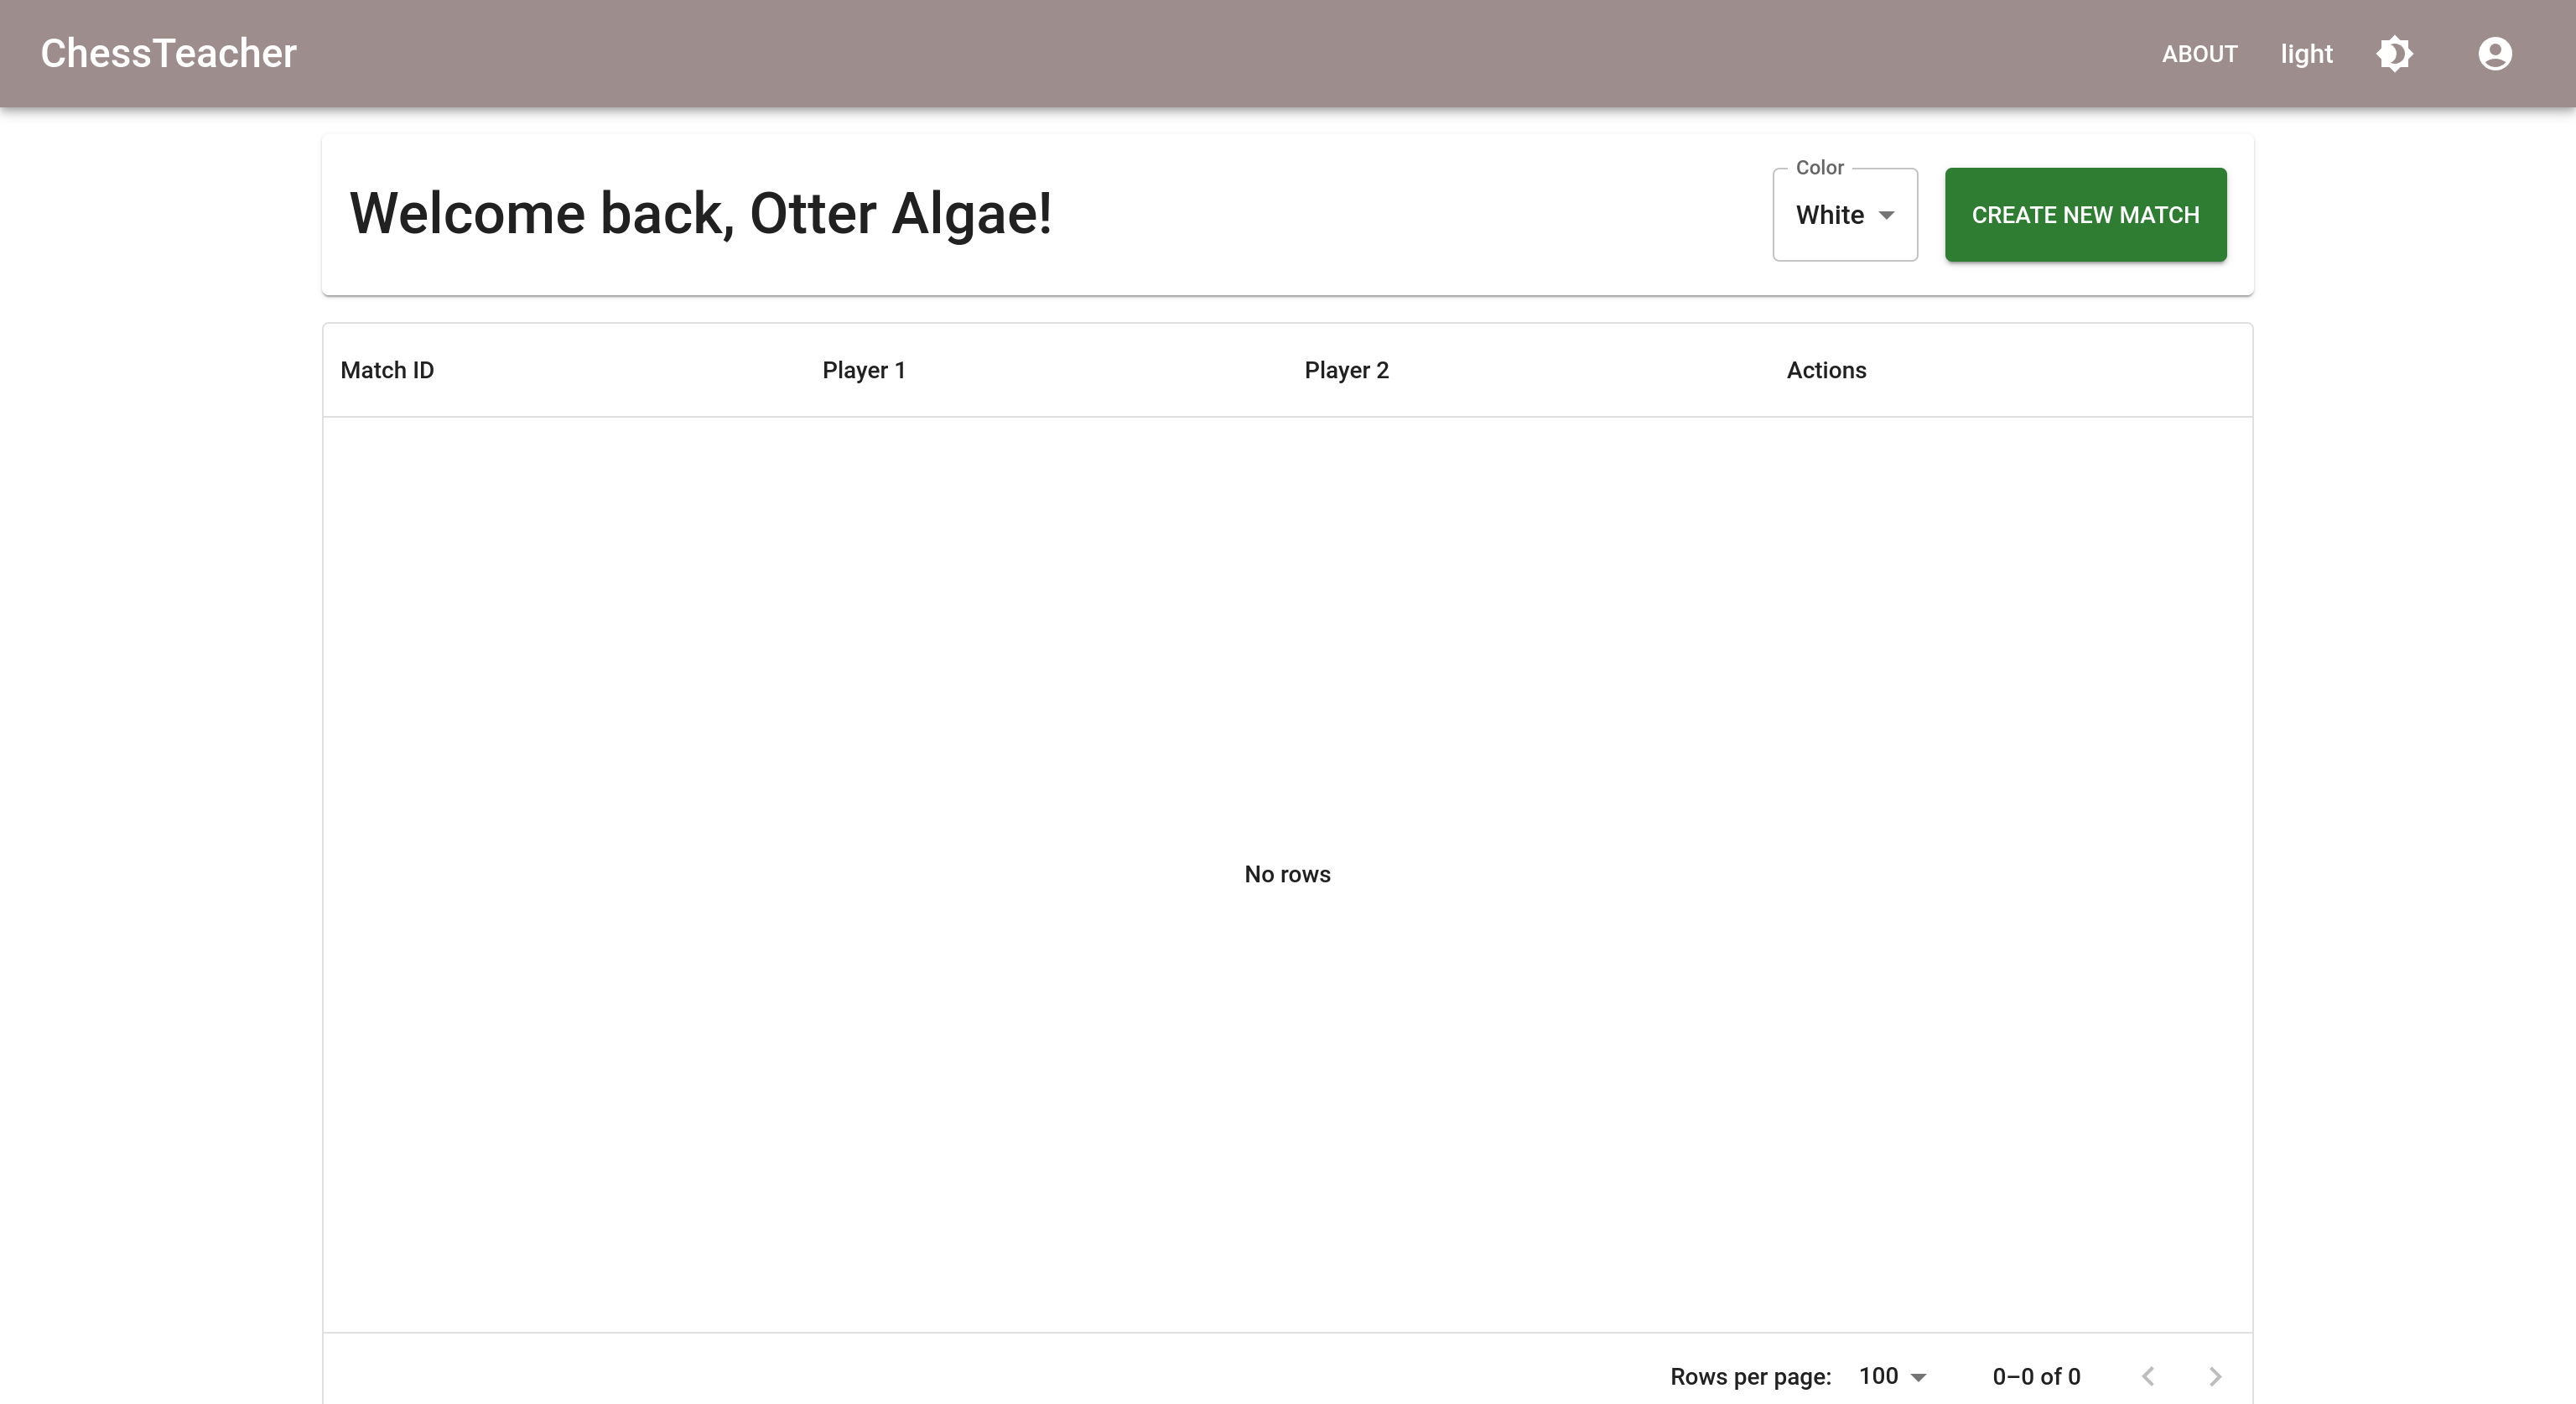
\includegraphics[width=1\textwidth]{frontend-lobby-empty}}
    \caption{The lobby listing of the website.}\label{fig:lobby-empty}
\end{figure}

\begin{figure}[H]
    \centering
    \setlength{\fboxsep}{0pt}
    \fbox{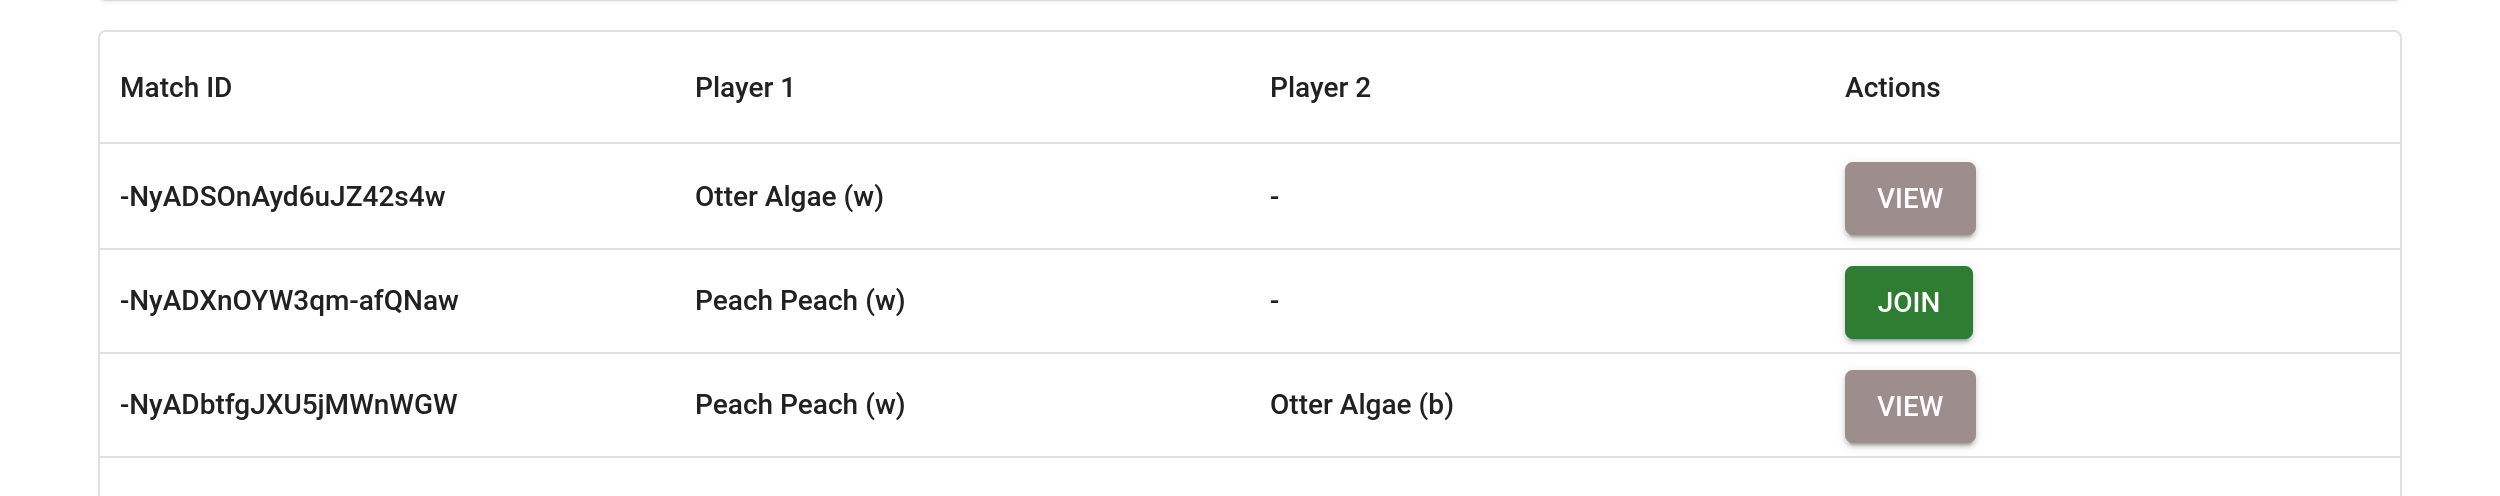
\includegraphics[width=1\textwidth]{frontend-lobby-game}}
    \caption{A game entry in the lobby.}\label{fig:lobby-game}
\end{figure}

\begin{figure}[H]
    \centering
    \setlength{\fboxsep}{0pt}
    \fbox{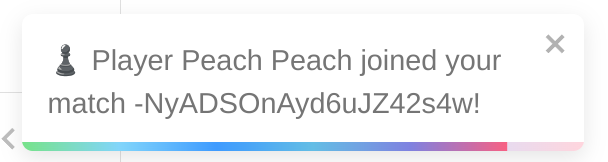
\includegraphics[width=0.7\textwidth]{frontend-lobby-join}}
    \caption{Notification when another player joins.}\label{fig:lobby-join}
\end{figure}
% textidote: ignore end

Once in-game, the players are greeted with a chessboard taking the majority of the screen, and a chat window to the
right of it, as seen in Figure~\ref{fig:game}.
The chessboard is the biggest element on the screen, as it is the main focus of the website, with the chat always
visible to the players.
The two players can take turns making moves, and the engine will provide feedback on the moves, as seen in
Figure~\ref{fig:game-chat}.
The engine gives both players the three best moves they can play on their turn.
Players and spectators can also chat with each other in the chat window.

% textidote: ignore begin
\begin{figure}[H]
    \centering
    \setlength{\fboxsep}{0pt}
    \fbox{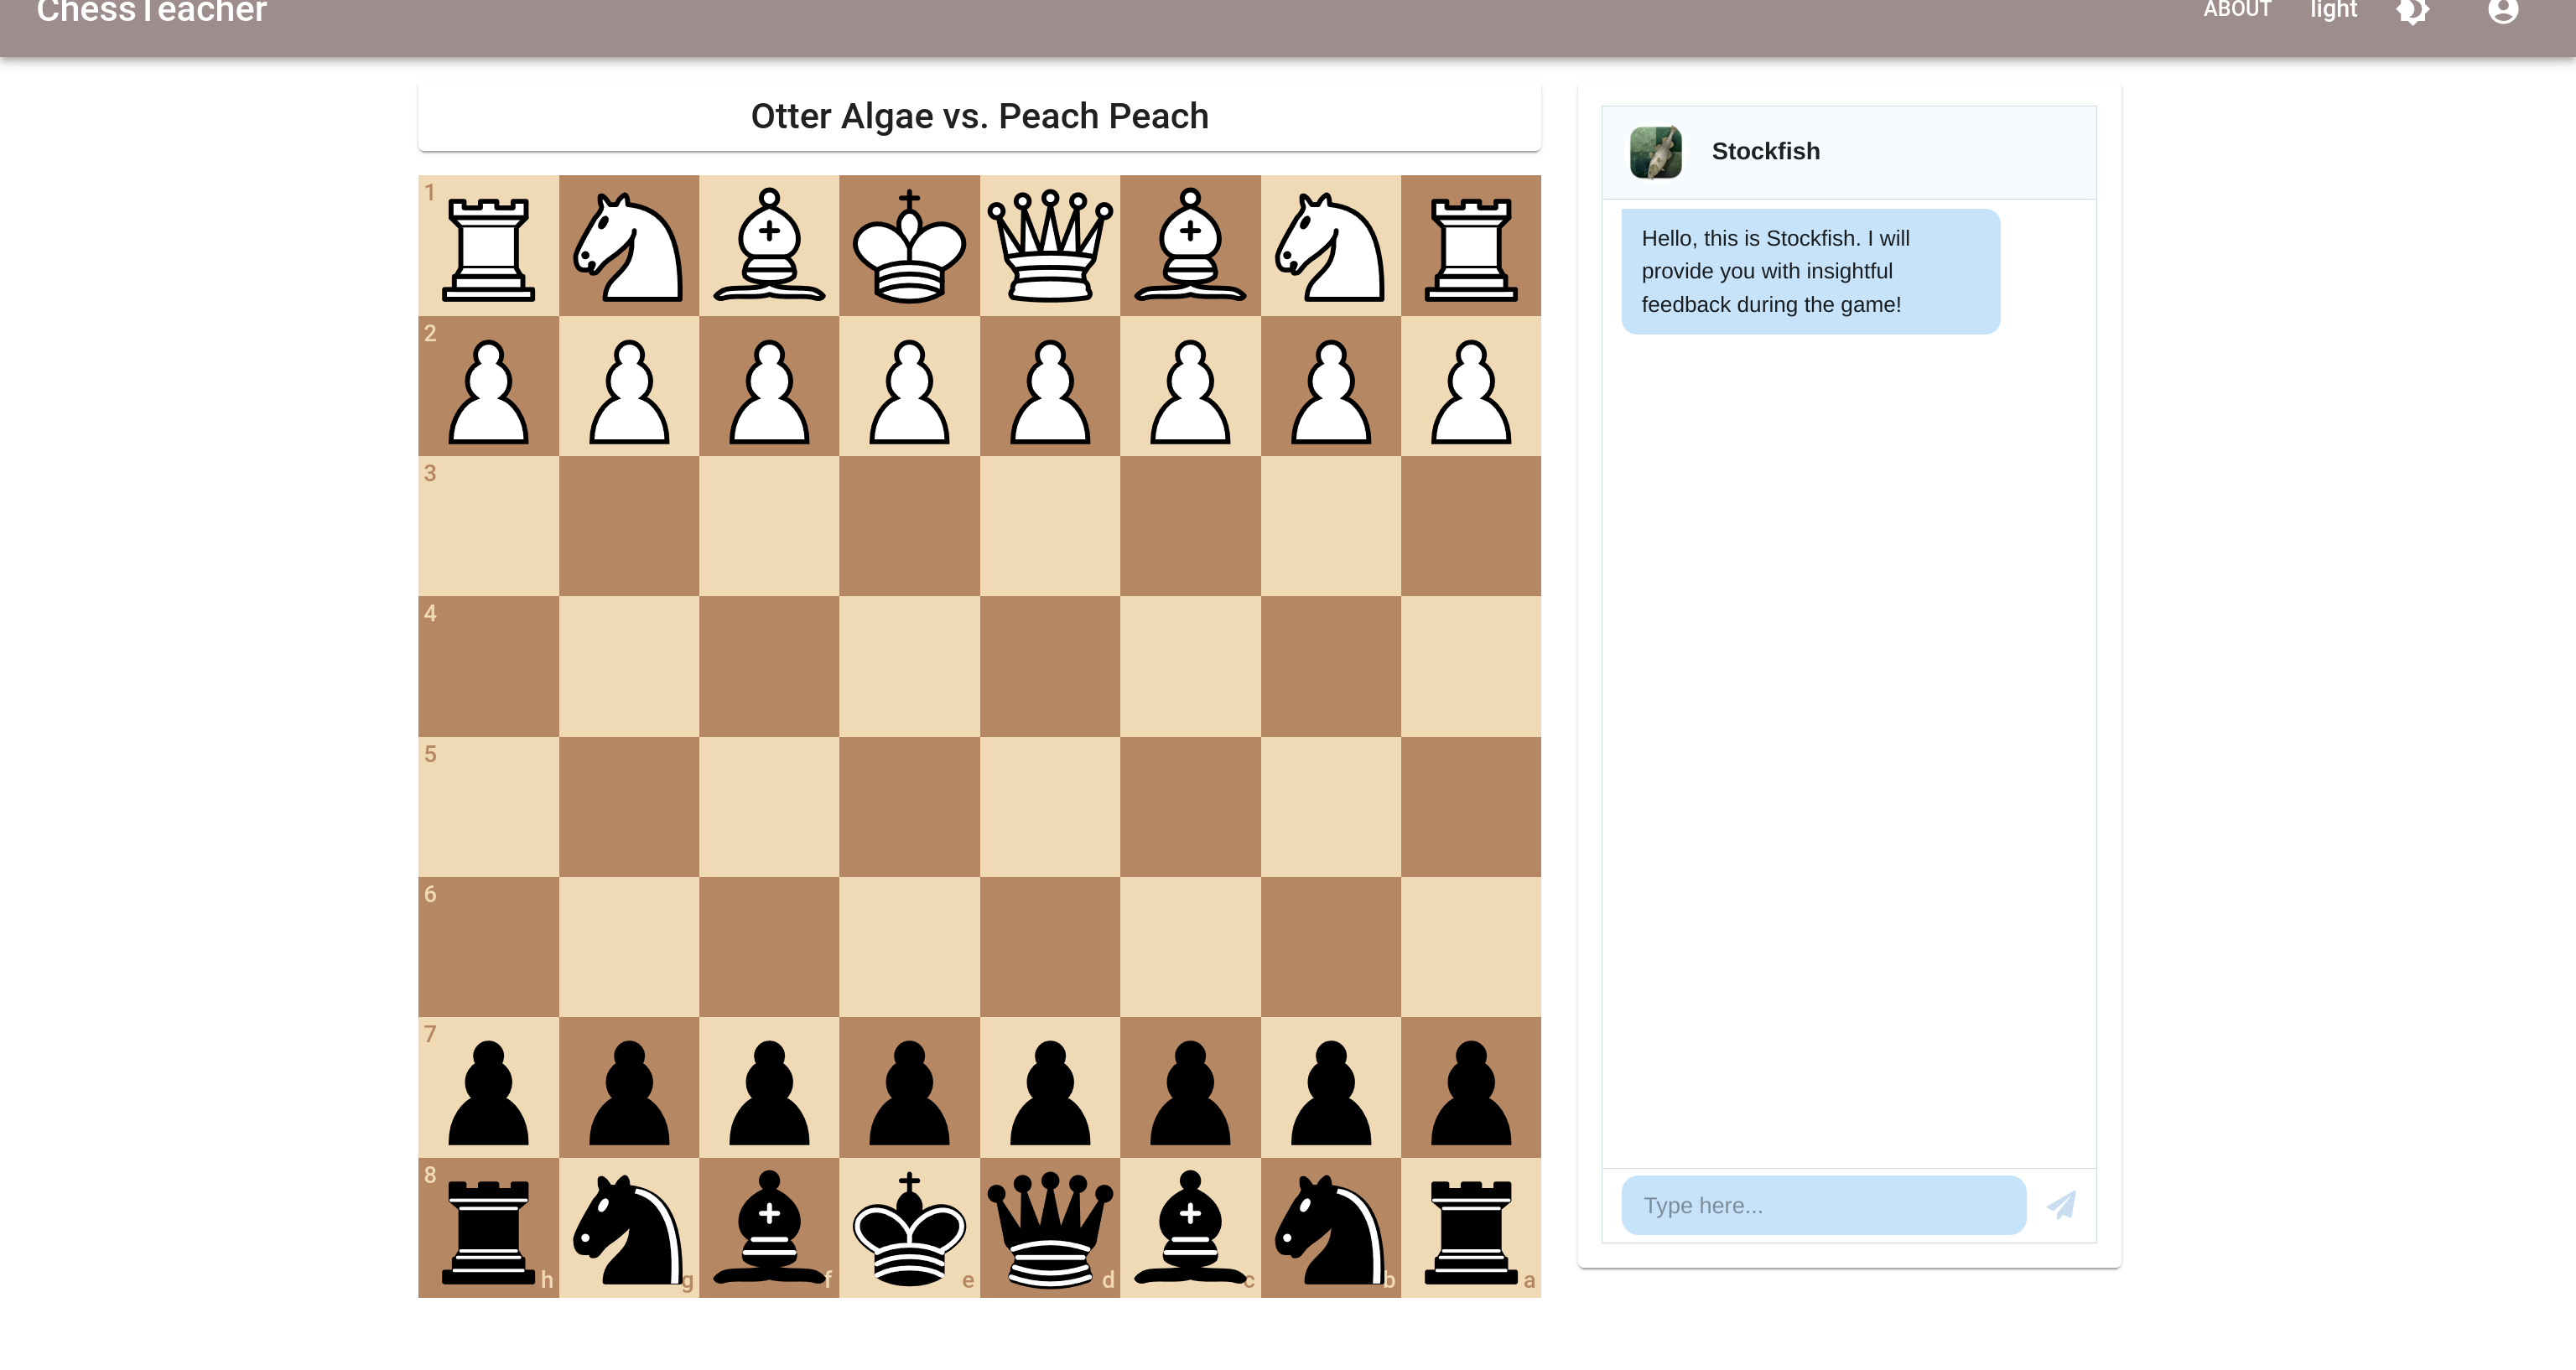
\includegraphics[width=1\textwidth]{frontend-game}}
    \caption{The in-game interface of the website.}\label{fig:game}
\end{figure}

\begin{figure}[H]
    \centering
    \setlength{\fboxsep}{0pt}
    \fbox{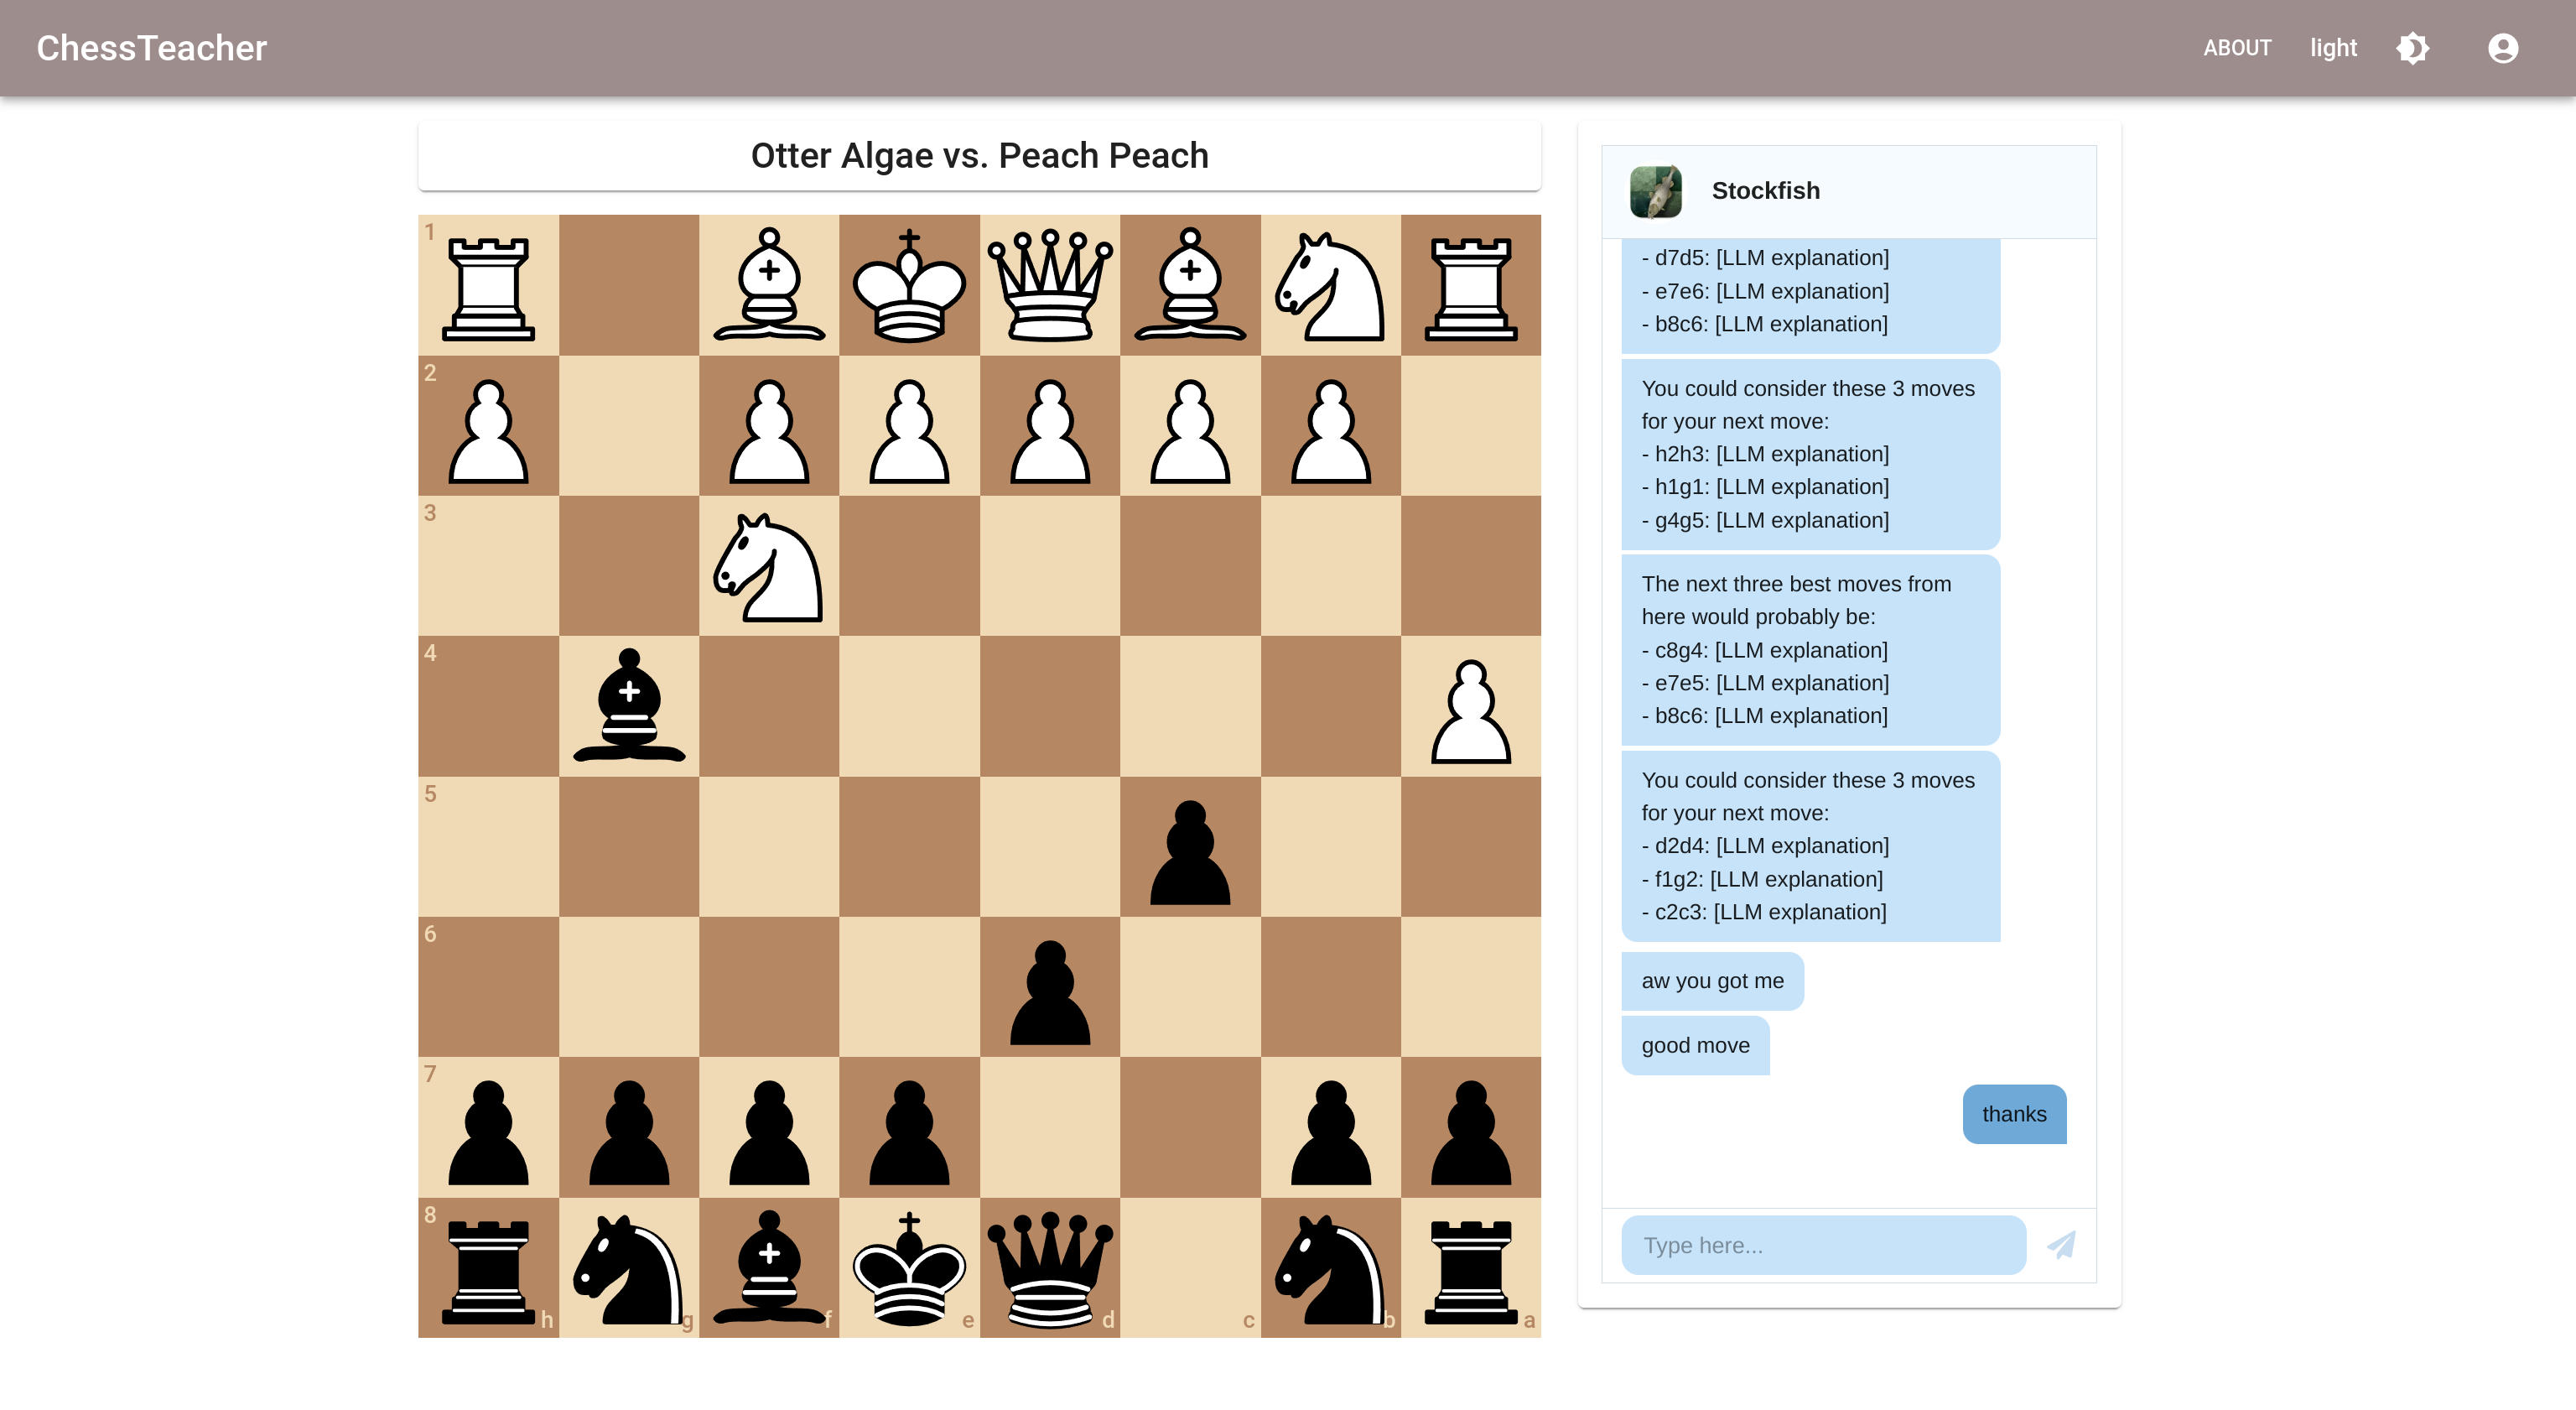
\includegraphics[width=1\textwidth]{frontend-game-chat}}
    \caption{A conversation between the players and stockfish.}\label{fig:game-chat}
\end{figure}
% textidote: ignore end

The website also has a dark mode, which can be toggled by clicking on the sun icon in the top right corner of the
website.
The option to change between light and dark mode was added to improve the user experience, as some users might prefer
one over the other.
The default mode is set to the user's system preference, but the user can change it to their liking.
The dark mode can be seen in Figure~\ref{fig:game-dark}.

% textidote: ignore begin
\begin{figure}[H]
    \centering
    \setlength{\fboxsep}{0pt}
    \fbox{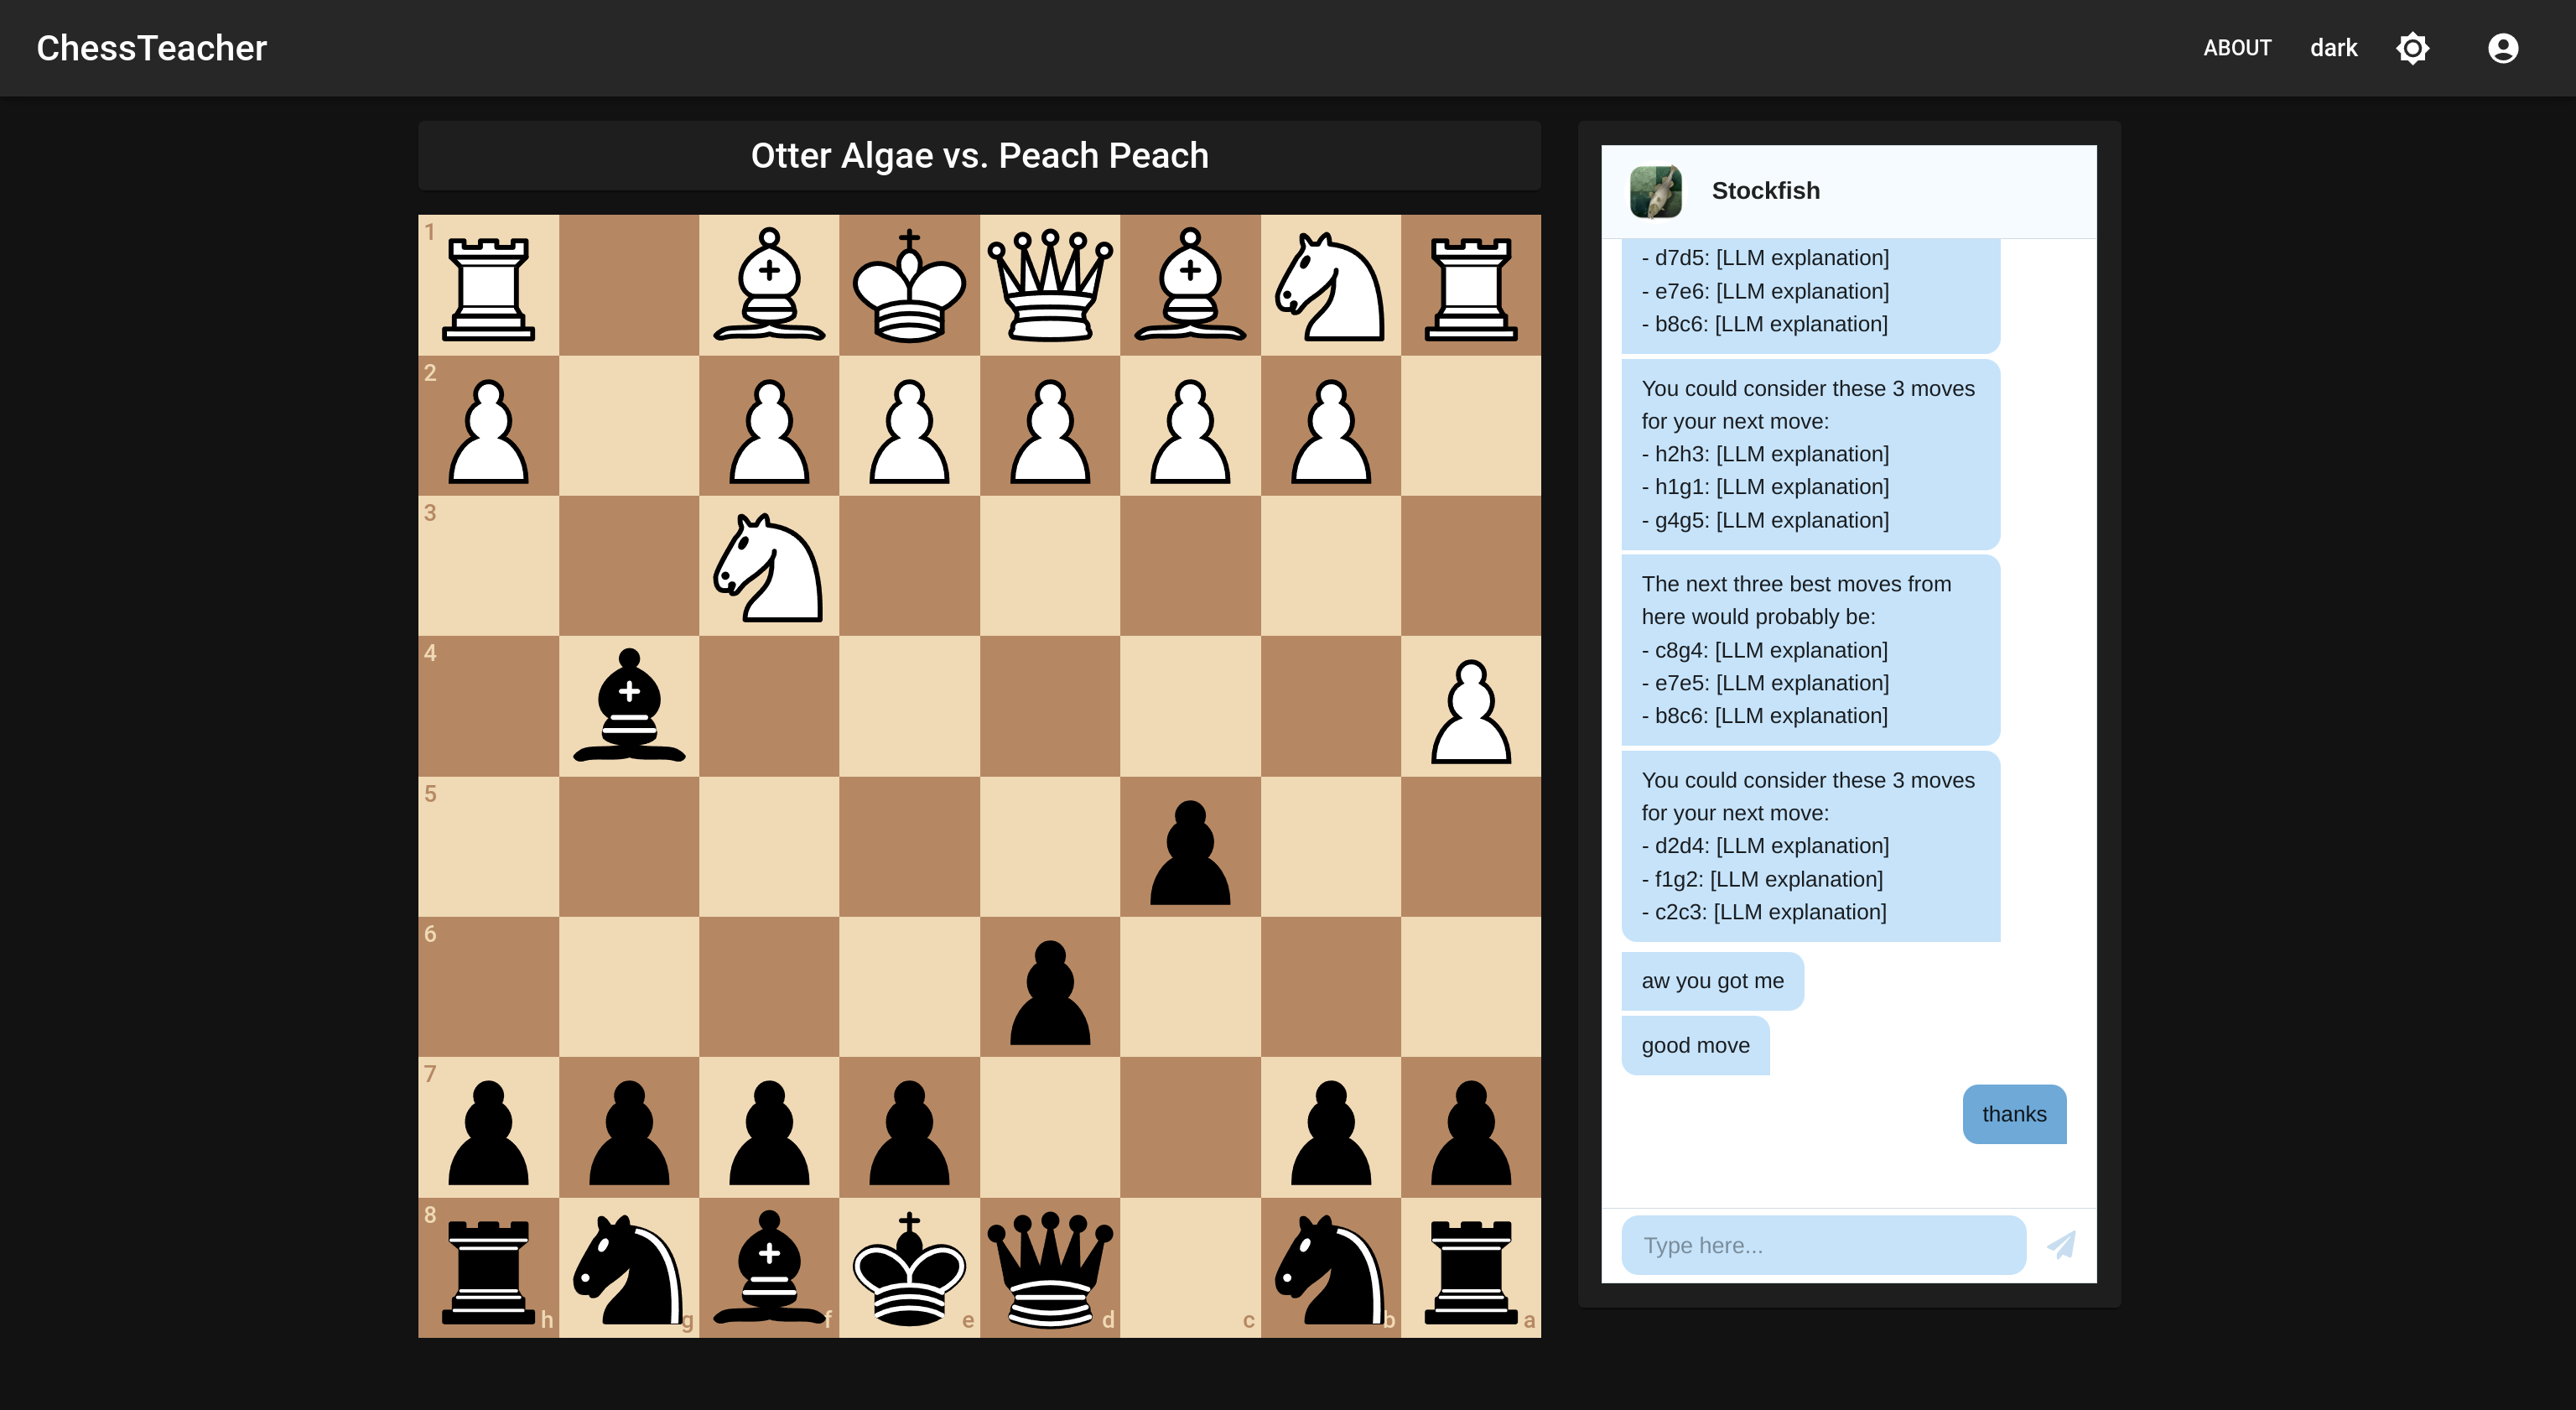
\includegraphics[width=1\textwidth]{frontend-game-dark}}
    \caption{The look of the website in dark mode.}\label{fig:game-dark}
\end{figure}
% textidote: ignore end

Apart from the lobby and the game interface, the website also has an account page, where the user can see their
personal information.
The account page can be seen in Figure~\ref{fig:account}.
It can be accessed by clicking on the user icon on the top right once logged in, and then clicking on ``Account''.
The profile picture is taken from the user's Google account, and if they don't have a picture, their initials will be
displayed instead.

% textidote: ignore begin
\begin{figure}[H]
    \centering
    \setlength{\fboxsep}{0pt}
    \fbox{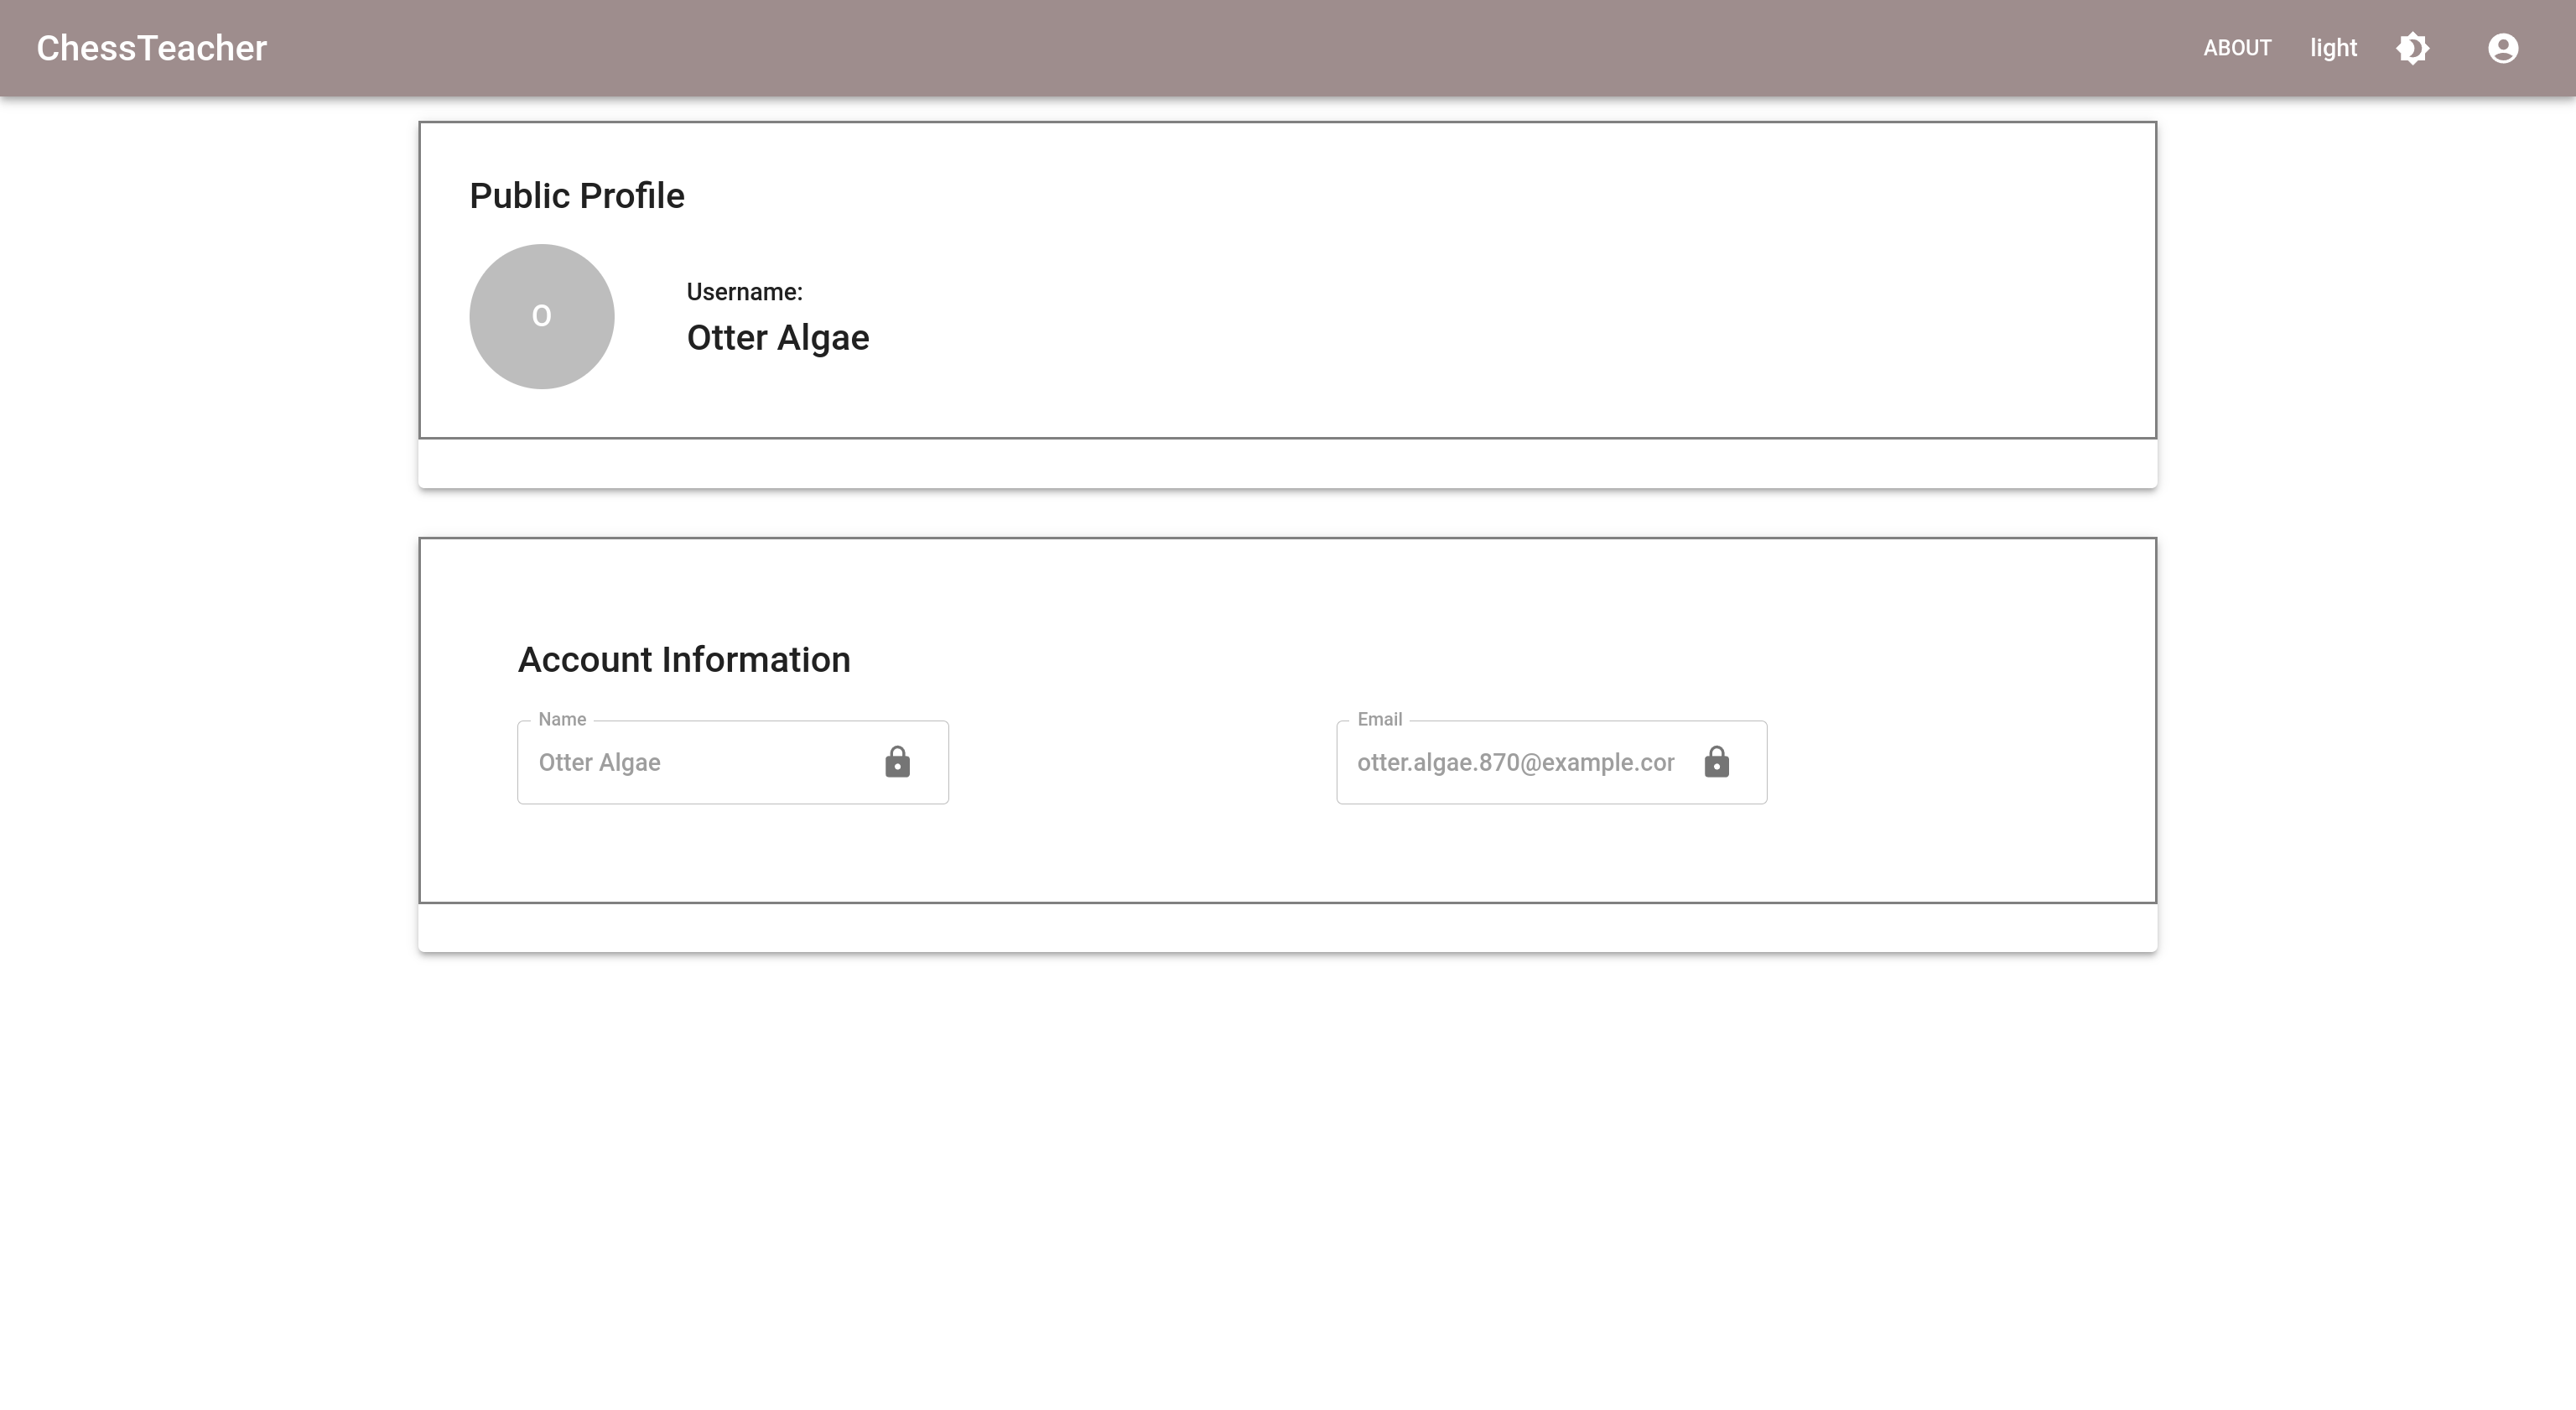
\includegraphics[width=1\textwidth]{frontend-account}}
    \caption{The account page of the website.}\label{fig:account}
\end{figure}
% textidote: ignore end

There is also an about page, which can be accessed by clicking on the ``About'' button on the top right of the
website.
It serves to inform the user about the project and the people behind it.
The page can be seen in Figure~\ref{fig:about}.

% textidote: ignore begin
\begin{figure}[H]
    \centering
    \setlength{\fboxsep}{0pt}
    \fbox{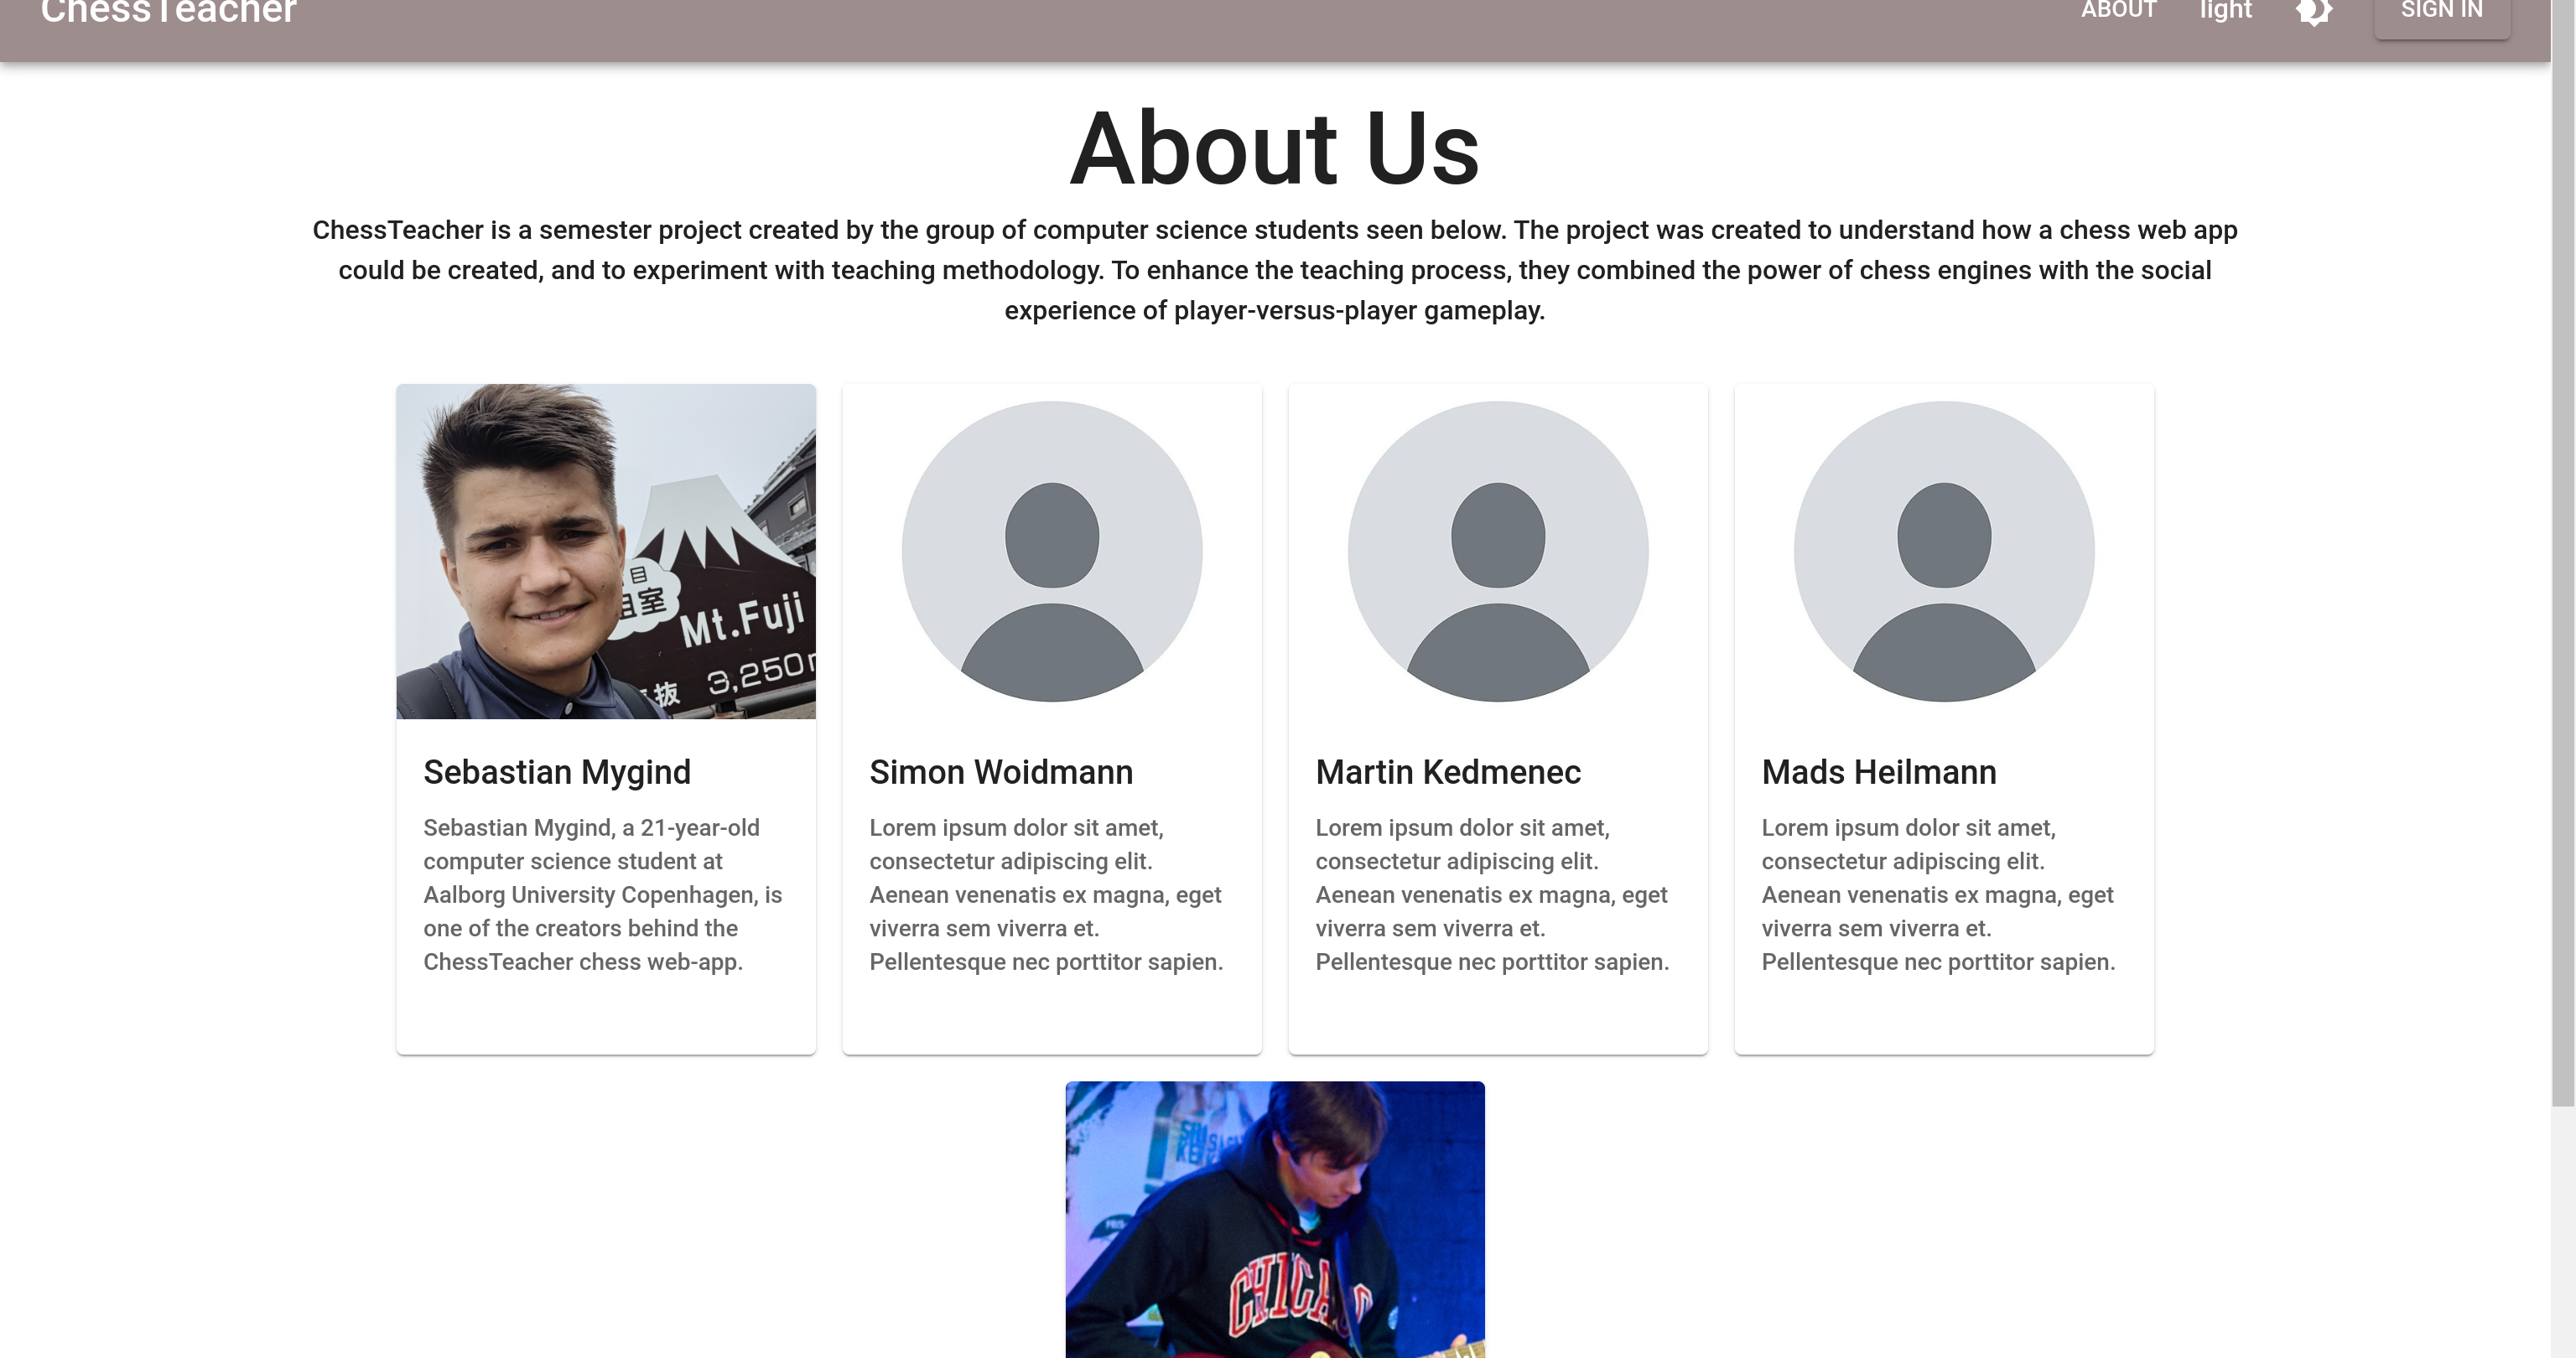
\includegraphics[width=1\textwidth]{frontend-about}}
    \caption{The about page of the website.}\label{fig:about}
\end{figure}
% textidote: ignore end

% textidote: ignore begin
\section{Back end}\label{sec:backend}
% textidote: ignore end

The back end of the application consists of multiple parts: A real-time NoSQL database~\cite{nosql}, authentication
database, Stockfish-powered REST API, and serverless edge functions.

In the following sections, we will take a more in-depth look at some of those components.

\subsection{Real-time database}\label{subsec:real-time-database}

The real-time database is provided through the Google Firebase Realtime Database~\cite{realtime-database} service.
This service provides an easy to integrate ``real-time database'', i.e., a database whose primary job is to synchronize
data between database clients, which, in our case, are the client front ends.
In other words, when data changes on one client, this data can easily be pushed to the remote cloud-hosted database,
which then, in turn, notifies the other clients of the data mutation.
This process ensures data synchronization between application clients.
It is achieved through the database's built-in WebSocket server, which lets the clients create a real-time connection
to the database.
The way that this feature is leveraged in our solution application is that it's used for updating the chessboard, lobby,
and chat states on each of the clients.
The chessboard piece state, without a doubt, has to be instantly synchronized between the players' and spectators'
clients, to create a smooth game experience.
The same goes for the in-game chat, and the lobby, which should show all the created and running matches in real time,
so that signed-in users easily can join or view a match.

\subsection{Stockfish API}\label{subsec:stockfish-api}

To fulfill the chess engine implementation requirement from the software requirement specification seen in
Section~\ref{sec:software-requirement-specification}, an instance of a chess engine needed to be added to the solution.
This presents various questions as e.g., what engine to use, and how to connect it with the rest of the solution.
The development team considered multiple options,
but settled on the Stockfish~\cite{stockfish} engine for a variety of reasons, which will be explained in the following
section.

\subsubsection{Rationale}

Stockfish is arguably one of the strongest chess engines~\cite{about-stockfish} on the market right now,
which makes it extremely desirable sheerly due to its processing power.
Stockfish has, since 2013, participated in the Top Chess Engine Championship (abbr.\ TCEC) and ``has finished first or
second in every season except one''~\cite{tcec-results,chess-com-stockfish},
and this result just proves Stockfish's capabilities.

% textidote: ignore begin % Due to `sh:d:002` on `\texttt{Chess.com}` and `\texttt{lichess.org}`
Furthermore, \texttt{Chess.com} and \texttt{lichess.org}, two of our main competitors, also extensively make use of
% textidote: ignore end
Stockfish in their own implementations~\cite{chess-com-stockfish,about-lichess}, which is another remarkable indicator
of Stockfish's capabilities and usage.

But arguably one of the most compelling reasons for using Stockfish is the fact that the engine is free and open source,
protected by the GPLv3 license~\cite{gplv3}.
The GPLv3 license is quite permissible, i.e., the user can freely use and even modify the original source code, as long
as the child software refers back to the license declaration and code repository of the licensed parent software.
In the case of the \texttt{ChessTeacher} software, it means that the addition of Stockfish is fully permissible within
the bounds of law.
The source code repository for Stockfish can be found on its official GitHub repository~\cite{github-stockfish}, from
where the source code can easily be downloaded and compiled using any C++-compatible compiler.

Those three main reasons compelled the software team to pick Stockfish as the driving chess engine for the back end.
In the following section, we will explain more concretely how Stockfish is connected to the rest of the software.

\subsubsection{Usage}

As Stockfish is binary executable software written in C++, it is not possible to run it in the browser,
unless it's compiled to WebAssembly~\cite{web-assembly}, which can natively run in modern browsers.
The WebAssembly approach was dropped in favor of a simpler REST API approach,
which features a simple Python script running in a containerized cloud environment.

As a brief overview; on receiving an HTTP request, the Python script calls a Stockfish wrapper library,
which in turn calls Stockfish and passes the response back to the Python script, which generates an HTTP response.
The reasons for choosing this architecture and data flow are multiple:
One of the core issues with the Stockfish software is that it outputs an overwhelming amount of plain text data to the
standard output stream when its built-in functions are called through its command line interface.
For our use case, we only require a few specific key data values from Stockfish to later display it on the browser front
end.
One solution to this problem would have been to execute Stockfish's CLI on the back end server, and stream its output
data directly to the front end over TCP or UDP\@.
Then, the data would have to be parsed and filtered on the front end, to extract the necessary data points.
The advantage of this method is that the developers would be able to keep using TypeScript for the programming of the
data processing as well as the other front end elements.
However, one of the disadvantages of this approach is that it uses a lot of network data when communicating the
information to the front end, which in turn is financially unsustainable.
Instead, the container server running Stockfish and the Python script parses the data locally and only returns the data
to the front end that is needed for the application to function.

The containerized environment to go with the script and Stockfish was created to ease the development and deployment
processes.
Containerized applications can easily be built and started for local development, and also easily be built and deployed
to the cloud.
For the cloud hosting of this container image, Google Cloud Run~\cite{google-cloud-run} was selected, as it features
a free tier for simple container images.
Reference is made to our Stockfish image in Appendix~\ref{ch:source-code-repositories} for the repository wherein the
source code for the image is contained.

To make sure the client is not waiting unnecessarily for the analysis of the position, while retaining some depth to the
board state analysis, the developers set a hard-coded midpoint of depth 8 for the Stockfish binary.

\subsection{Stockfish API functions}\label{subsec:stockfish-api-functions}

The two main functionalities of the script are the functions \texttt{evaluate\_position} and \texttt{analyze\_move}.

The position is as before mentioned communicated through a FEN (Forsyth-Edwards Notation) string.
The FEN string is produced by the frontend and is included in the request for the position evaluation.

% textidote: ignore begin

\subsubsection{Function: \texttt{evaluate\_position}}\label{subsubsec:function:evaluate_position}
% textidote: ignore end

This function's main purpose is to evaluate a FEN position.
The FEN position is then evaluated by Stockfish.
A snippet of the function can be seen in Listing~\ref{lst:main.py-evaluate_position}, where the function definition is
listed.

\begin{lstlisting}[
    style=pythonStyle,
    label={lst:main.py-evaluate_position},
    caption={Definition of function \texttt{evaluate\_position} in \texttt{main.py}},
    captionpos=b,
]
@app.post("/evaluate-position")
async def evaluate_position(
    evaluate_position_request: EvaluatePositionRequest,
) -> DataResponse[EvaluatePositionResponse]:
\end{lstlisting}

In the definition, it can be seen that the function has a single formal parameter \texttt{evaluate\_position\_request},
which is of type \texttt{EvaluatePositionRequest}, which encapsulates a FEN string and a time tracking variable.
It returns an object of type \texttt{EvaluatePositionResponse}, which contains an evaluation of the FEN position,
statistics regarding whether the game was won, drawn or lost, and a list of the top three recommended moves.

% textidote: ignore begin

\subsubsection{Function: \texttt{analyze\_move}}\label{subsubsec:function:analyze_move}
% textidote: ignore end

This function's main purpose is to analyze a single move.
A snippet of the function can be seen in Listing~\ref{lst:main.py-analyze_move}, where the function definition is
listed.

\begin{lstlisting}[
    style=pythonStyle,
    label={lst:main.py-analyze_move},
    caption={Definition of function \texttt{analyze\_move} in \texttt{main.py}},
    captionpos=b,
]
@app.post("/analyze-move")
async def analyze_move(
    analyze_move_request: AnalyzeMoveRequest,
) -> DataResponse[AnalyzeMoveResponse]:
\end{lstlisting}

As before, in the definition, it can be seen that the function has a single formal parameter
\texttt{analyze\_move\_request}, which is of type \texttt{AnalyzeMoveRequest}, which encapsulates a FEN string and a
time tracking variable.
In addition to that, it also encapsulates a move string, wherein the move to be analyzed is located.
It returns an object of type \texttt{AnalyzeMoveResponse}.
This object contains an evaluation of the board state after the move is made, whether the move was a capture or not,
and the absolute change in evaluation between the pre- and post-move board positions.

\subsection{Unit testing}\label{subsec:unit-testing}
When creating the functions for the REST API, unit tests were created to ensure that the functions worked as intended.
The unit tests were created using FASTAPI's built-in testing functionality called \texttt{TestClient}.

\begin{lstlisting}[
    style=pythonStyle,
    label={lst:test_main.py-evaluate_position},
    caption={Test of \texttt{evaluate-position} in \texttt{test\_main.py}},
    captionpos=b,
]
def test_evaluate_position():
    response = client.post(
        "/evaluate-position",
        json={"fen": "rnbqkbnr/pppppppp/8/8/8/8/PPPPPPPP/RNBQKBNR w KQkq - 0 1"},
    )
    assert response.status_code == 200
\end{lstlisting}

In Listing~\ref{lst:test_main.py-evaluate_position}, a test of the \texttt{evaluate-position} function is shown.
The test uses a client object to send a POST request to the \texttt{evaluate-position} endpoint with a FEN string as
the payload.
The test then asserts that the response status code is 200, which means that the request was successful.

The purpose of this test is to first ensure that the \texttt{/evaluate-position} endpoint is reachable and can process
requests.
Secondly, it ensures that the endpoint can handle a FEN string as input and return a response.
Lastly, it ensures that the response status code is 200, which means that the request was successful.

\pagebreak

Below is an example of a test that checks if the endpoint returns a status code of 400 when an invalid FEN
string is provided.

\begin{lstlisting}[
    style=pythonStyle,
    label={lst:test_main.py-evaluate_position-invalid-fen},
    caption={Test of \texttt{evaluate-position} in \texttt{test\_main.py} for invalid FEN string},
    captionpos=b,
]
def test_evaluate_position_invalid_fen():

    response = client.post("/evaluate-position", json={"fen": "fen-position"})

    assert response.status_code == 400
    assert response.json() == {"detail": "Invalid FEN"}
\end{lstlisting}

In Listing~\ref{lst:test_main.py-evaluate_position-invalid-fen}, a test of the \texttt{evaluate-position} function is
shown.
%textidote: ignore begin
The purpose of this test is to ensure the endpoint returns a status code of 400 and a JSON response with the
%textidote: ignore end
%textidote: ignore begin
message \texttt{''Invalid FEN''} when an invalid FEN string is provided.
%textidote: ignore end
This ensures that the endpoint can handle invalid input and return an appropriate error response.


    \chapter{Usability Testing}\label{ch:user-test}

After the development of the website and the game,
the team conducted usability testing to gather feedback on the project.
This feedback would be used to improve the website and game before the final release.
It could also provide the team with insights into the user experience and the game's playability.


\section{Methodology}\label{sec:methodology}

The tests were conducted by multiple members of the team, so to keep the results consistent, a methodology was
established.
It consisted of a script that the team members followed, ensuring that the same questions were asked to each
participant.
The script was divided into four parts: introduction, user interface and experience, gameplay, and feedback.
The parts were designed like an interview, where the team members would first show them the aspects of the website,
then let them play the game for themselves, and finally ask a series of questions to gather their feedback.
The results in Section~\ref{sec:results} are based on their feedback rather than the script.


\section{Participants}\label{sec:participants}

A total of three participants were recruited for the usability testing.
They varied between age and skill level, with at least two of them fitting the target audience of the game.
This section will introduce the participants and their background.

\begin{itemize}

    \item \textbf{Ronja} is 22 years old, and she ranks at 800 ELO, which fits in the target audience of beginners.
    She was taught to play in her kindergarten, and now she plays chess occasionally for fun.

    \item \textbf{Clara} is 19 years old, and she ranks at 1000 ELO, which also fits in the target audience.
    She studies machine learning, so she could provide valuable feedback on the Stockfish implementation.
    She was taught to play chess in an academic setting.

    \item \textbf{Peter} is 31 years old, and his ranks is 1700 ELO, which is above the target audience.
    He plays chess semi-professionally, first learning to play from his father and then in school.
    % textidote: ignore begin % due to chess.com
    He got more interested in chess during the pandemic due to Chess.com's popularity and chess' presence on Twitch.
    % textidote: ignore end
    While he may not be the target audience, his experience should provide the team with valuable feedback.

\end{itemize}

% textidote: ignore begin % due to section being too short


\section{Results}\label{sec:results}
% textidote: ignore end

The results of the test are based on the feedback from the participants.
The feedback was divided into three categories similar to the methodology: interface and experience, gameplay, and
feedback.
Each of these categories will have a mixture of all participants' feedback, providing a comprehensive view of the user
test.

\subsection{Interface and experience}\label{subsec:ui/ux}

The overall feedback on the interface was positive.
Everyone thought that the website was visually appealing, calling it pretty.
The team did however receive some constructive criticism.

Peter pointed out that the front page was not intuitive and Clara suggested that the buttons should be larger, labelled,
and link together.
Peter also mentioned that it was difficult to figure out how to play, he proposed that the About page should contain
information on how to create an account and what the website is about.

The in-game interface was also critiqued.
Clara noted that the Stockfish feedback lacked visual cues, her idea was that there should be arrows on the chessboard,
which is something that the team had previously discussed.
Peter mentioned that the notations provided by Stockfish were incorrect and complained about the lack of sound effects
and there being no apparent indication for when a game is over.
Meanwhile, Ronja thought that nothing was missing.

\subsection{Gameplay}\label{subsec:gameplay}

The users critiqued the gameplay, with the main focus being on the Stockfish implementation.
Clara thought that the Stockfish feedback was too direct, suggesting that it should give smaller hints instead of the
direct solution.
Peter mentioned that the feedback should provide future moves along with the current move.
Ronja didn't immediately understand what the Stockfish feedback was, but after using Stockfish a little, she lost
interest in it.
This indicates that the current Stockfish implementation has a lot of room for improvement on what feedback it provides
and how to provide it to the player.

Clara also mentioned that the game should have more teaching tools, such as puzzles and guides to how to play chess.
The team considered these features given the learning nature of the game, but there are already existing solutions that
provide them, so they were not prioritized, instead focusing on the coaching aspect of the game.

Lastly, the users were asked about the idea of using machine learning along with Stockfish to provide feedback.
The rationale behind this question was due to a prior discussion within the team, which will be later discussed in
Section~\ref{sec:large-language-model-implementation}.
Clara and Ronja both liked the idea of using machine learning, while Peter was more skeptical.
He did not particularly like the idea due to the lack of control over the large language model's answers, so the team
cannot be guaranteed that it'll provide correct information.
Clara however thinks that in combination with Stockfish it could provide accurate information whilst also giving more
natural responses and explanations.

% textidote: ignore begin % due to section being too short

\subsection{Feedback}\label{subsec:feedback}
% textidote: ignore end

To conclude the usability testing, the participants were asked to provide their final thoughts on the project, from the
idea to the execution.
Peter's thoughts are a little mixed.
Ronja had a positive experience, but only after she understood how to use Stockfish.
Clara thinks that the website can motivate beginners to play chess, and she wishes that she used an engine like
Stockfish
at the academy where she learned to play chess.
% textidote: ignore begin % due to chess.com
She and Ronja would use the website again, but Peter would rather use alternatives like Chess.com and Lichess, because
he believes that they can do everything our website can do and more.
% textidote: ignore end

% textidote: ignore begin % due to section being too short


\section{Conclusion}\label{sec:tests-conclusion}
% textidote: ignore end

The feedback from the users was generally positive, but there are still areas that need improvement.
The team received a lot of suggestions for areas to improve, some of which were already discussed prior to the user
tests, but also some new ones.
For example, expanding the About page to include information on how to create an account and what the website is about.
The team already knew what it's about, but had not considered that new users might not.
Another example is the wrong notations provided by Stockfish, which the team was not aware of.
Feedback on the Stockfish implementation was also valuable, but some suggestions could not be implemented due to time
constraints.
Overall, the usability testing was a success,
and the feedback provided valuable insights for the team on how to improve the website and game before the final
release.

    % textidote: ignore begin
\chapter{Discussion}\label{ch:discussion}
% textidote: ignore end

% textidote: ignore begin
\section{Software requirements evaluation}\label{sec:software-requirements-evaluation}
% textidote: ignore end

This section refers back to Section~\ref{sec:software-requirement-specification} and more specifically
Table~\ref{tab:srs}.

% textidote: ignore begin

\subsection{Must-haves}\label{subsec:must-haves}
% textidote: ignore begin

This section concerns the evaluation of the must-have requirements.
Most must-have requirements are satisfied in the development of the first release of the ChessTeacher project.
This entails the basic chess functionality, the online multiplayer functionality and the chess engine implementation.
They work seamlessly and efficiently and are well integrated into the overall project.

% textidote: ignore begin

\subsubsection{Applied learning principles}
% textidote: ignore begin

Though most features are well implemented as mentioned above, there are some missing features.
The project is missing some key features regarding the learning principles mentioned in
Section~\ref{sec:learning-methods-for-chess}.
Key missing features include explanations and interactivity.
As chess as a game is complex, there are too many different positions for it to make sense to hard-code responses for
different positions.
To reach the full potential of the idea, the project needs some form of dynamic language model that is able to interpret
the Stockfish provided feedback, process this information and provide tailored feedback to the user.
This implementation is further discussed in Section~\ref{sec:large-language-model-implementation}.
These key missing features make for worse initial feedback by the test subjects as further discussed in
Section~\ref{sec:results}.
Even though this is undesired feedback and functionality for the overall potential of a chess learning web
application, the developers are still satisfied with the result.

% textidote: ignore begin

\subsubsection{Complex chess rules}
% textidote: ignore begin

Another feature that has not been included is the time control rule of chess.
Chess is usually played with time restrictions, no matter which variant of chess is in question, i.e.\ international,
blitz, rapid, bullet, etc.
Even though time control is a vital game mechanic in chess both competitively and on an amateur level it has not been
implemented, as the purpose of the web application is to learn chess rather than to play chess.
Individuals may dislike a timer counting them down whilst trying to learn chess, which is an argument for not
implementing the feature.
However, it is also important to learn where and when in the game to spend one's time thinking; why one could argue that
it should have been implemented to support learning of time management in chess.

% textidote: ignore begin

\subsection{Should-haves}\label{subsec:should-haves}
% textidote: ignore begin

This section concerns the evaluation of the should-have requirements.
Once again, most should-have requirements are satisfied in the development of the first release of the ChessTeacher
project.
This entails the implementation of user accounts, user registration and authentication, chat functionality and game
listing.
As the previous requirements, the mentioned factors all work efficiently and smoothly,
as also supported by the usability tests.

% textidote: ignore begin

\subsubsection{Engine feedback in English}
% textidote: ignore begin

However, the english feedback from Stockfish is, as per the first release of the project, hard-coded to be a random
message from a selection of three constructed sentences.
This is due to the same reasons as mentioned in Section~\ref{subsec:must-haves}.
Even though the implementation of the english user feedback is suboptimal, it still functions as desired when accounting
for the time and experience limitations.

Another implementation not prioritized due to time constraints is the front-end implementation of the
\verb|analyze_move| function mentioned in Section~\ref{subsec:stockfish-api-functions}.
Implementing the functionality would serve even more feedback to the user about their move.
This can help them improve and learn as mentioned in Section~\ref{subsec:assisted-learning}.

% textidote: ignore begin
\section{Large language model implementation}\label{sec:large-language-model-implementation}
% textidote: ignore end

As mentioned in Section~\ref{subsec:must-haves}, some key features, hereby explanations and interactivity, are not
implemented in the first release of the ChessTeacher project.
This makes for an application that in the current state may not suffice to resolve the problem statement.
There are several reasons for this gap and this section will discuss a possible solution to this issue.

Artificial intelligence (AI) has seen a significant increase in popularity in recent years, with the development of
large language models (LLMs) being one of the most notable advancements.
LLMs provide a way to generate human-like text, which can be used in a variety of applications, with chatbots being a
popular example.
As the core concept of this project is replacing a human chess coach with a computer, LLMs could be a valuable addition.

A potential use case for an LLM in the project could be to provide explanations for the moves suggested by Stockfish.
Currently, the user is given the three best moves without any explanation as to why they are the best.
By using an LLM, the user could ask follow-up questions to the feedback, and the LLM could provide a more detailed
explanation.
An example of this interaction can be seen in Figure~\ref{fig:llm}.

% textidote: ignore begin
\begin{figure}[H]
    \centering
    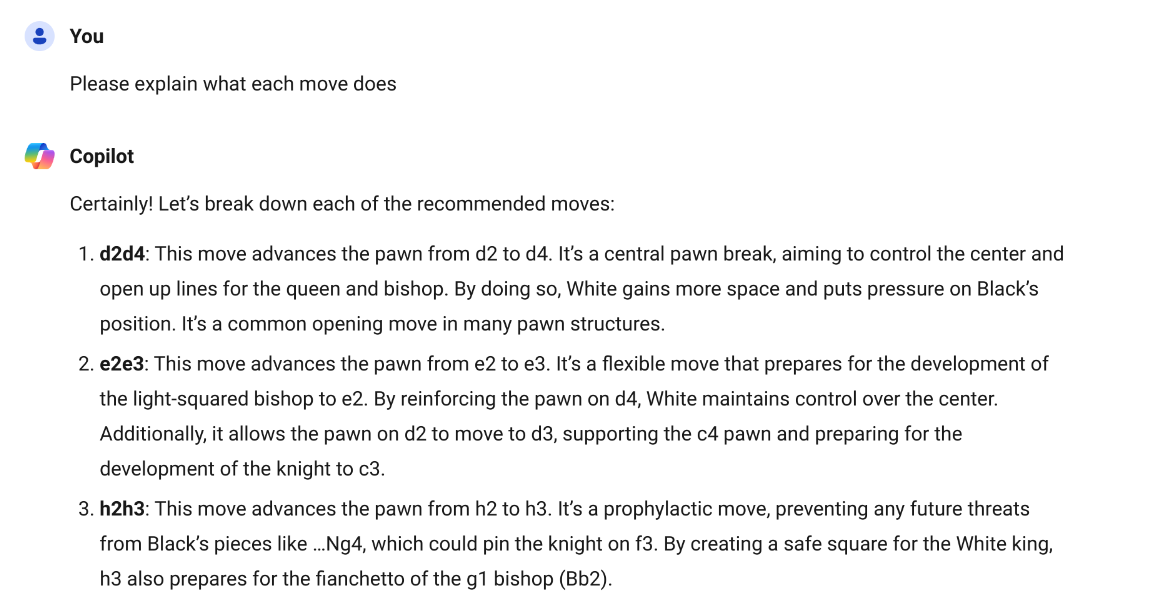
\includegraphics[width=0.85\textwidth]{llm}
    \caption{Example of a conversation with an LLM.}\label{fig:llm}
\end{figure}
% textidote: ignore end

It is important to note that LLM models are not perfect, and there are some potential issues that could arise from
implementing one.
The main concern is that the LLM could provide incorrect information, which could be detrimental to the learning
experience.
ChatGPT, a popular LLM, is known for its inability to actually play chess, as it often makes illegal
moves~\cite{llm-chess}.
The team however believes that Stockfish could be used in conjunction with the LLM to ensure that the information
provided is correct.
That would solve the issue of incorrect information, but it would also require a substantial amount of work.

The team did consider using an LLM during the planning phase of the project, but ultimately decided against it.
The main reason was because the team expected that Stockfish would provide a sufficient level of interactivity for the
users.
However, as evident from the usability testing results in Section~\ref{sec:results}, the feedback from Stockfish was
not able to contribute to the learning experience as much as the team had hoped.
Reflecting on this, the team believes that an LLM could be a valuable addition to the project, and should be implemented
if the project were to be expanded.

% textidote: ignore begin
\begin{figure}[H]
    \centering
    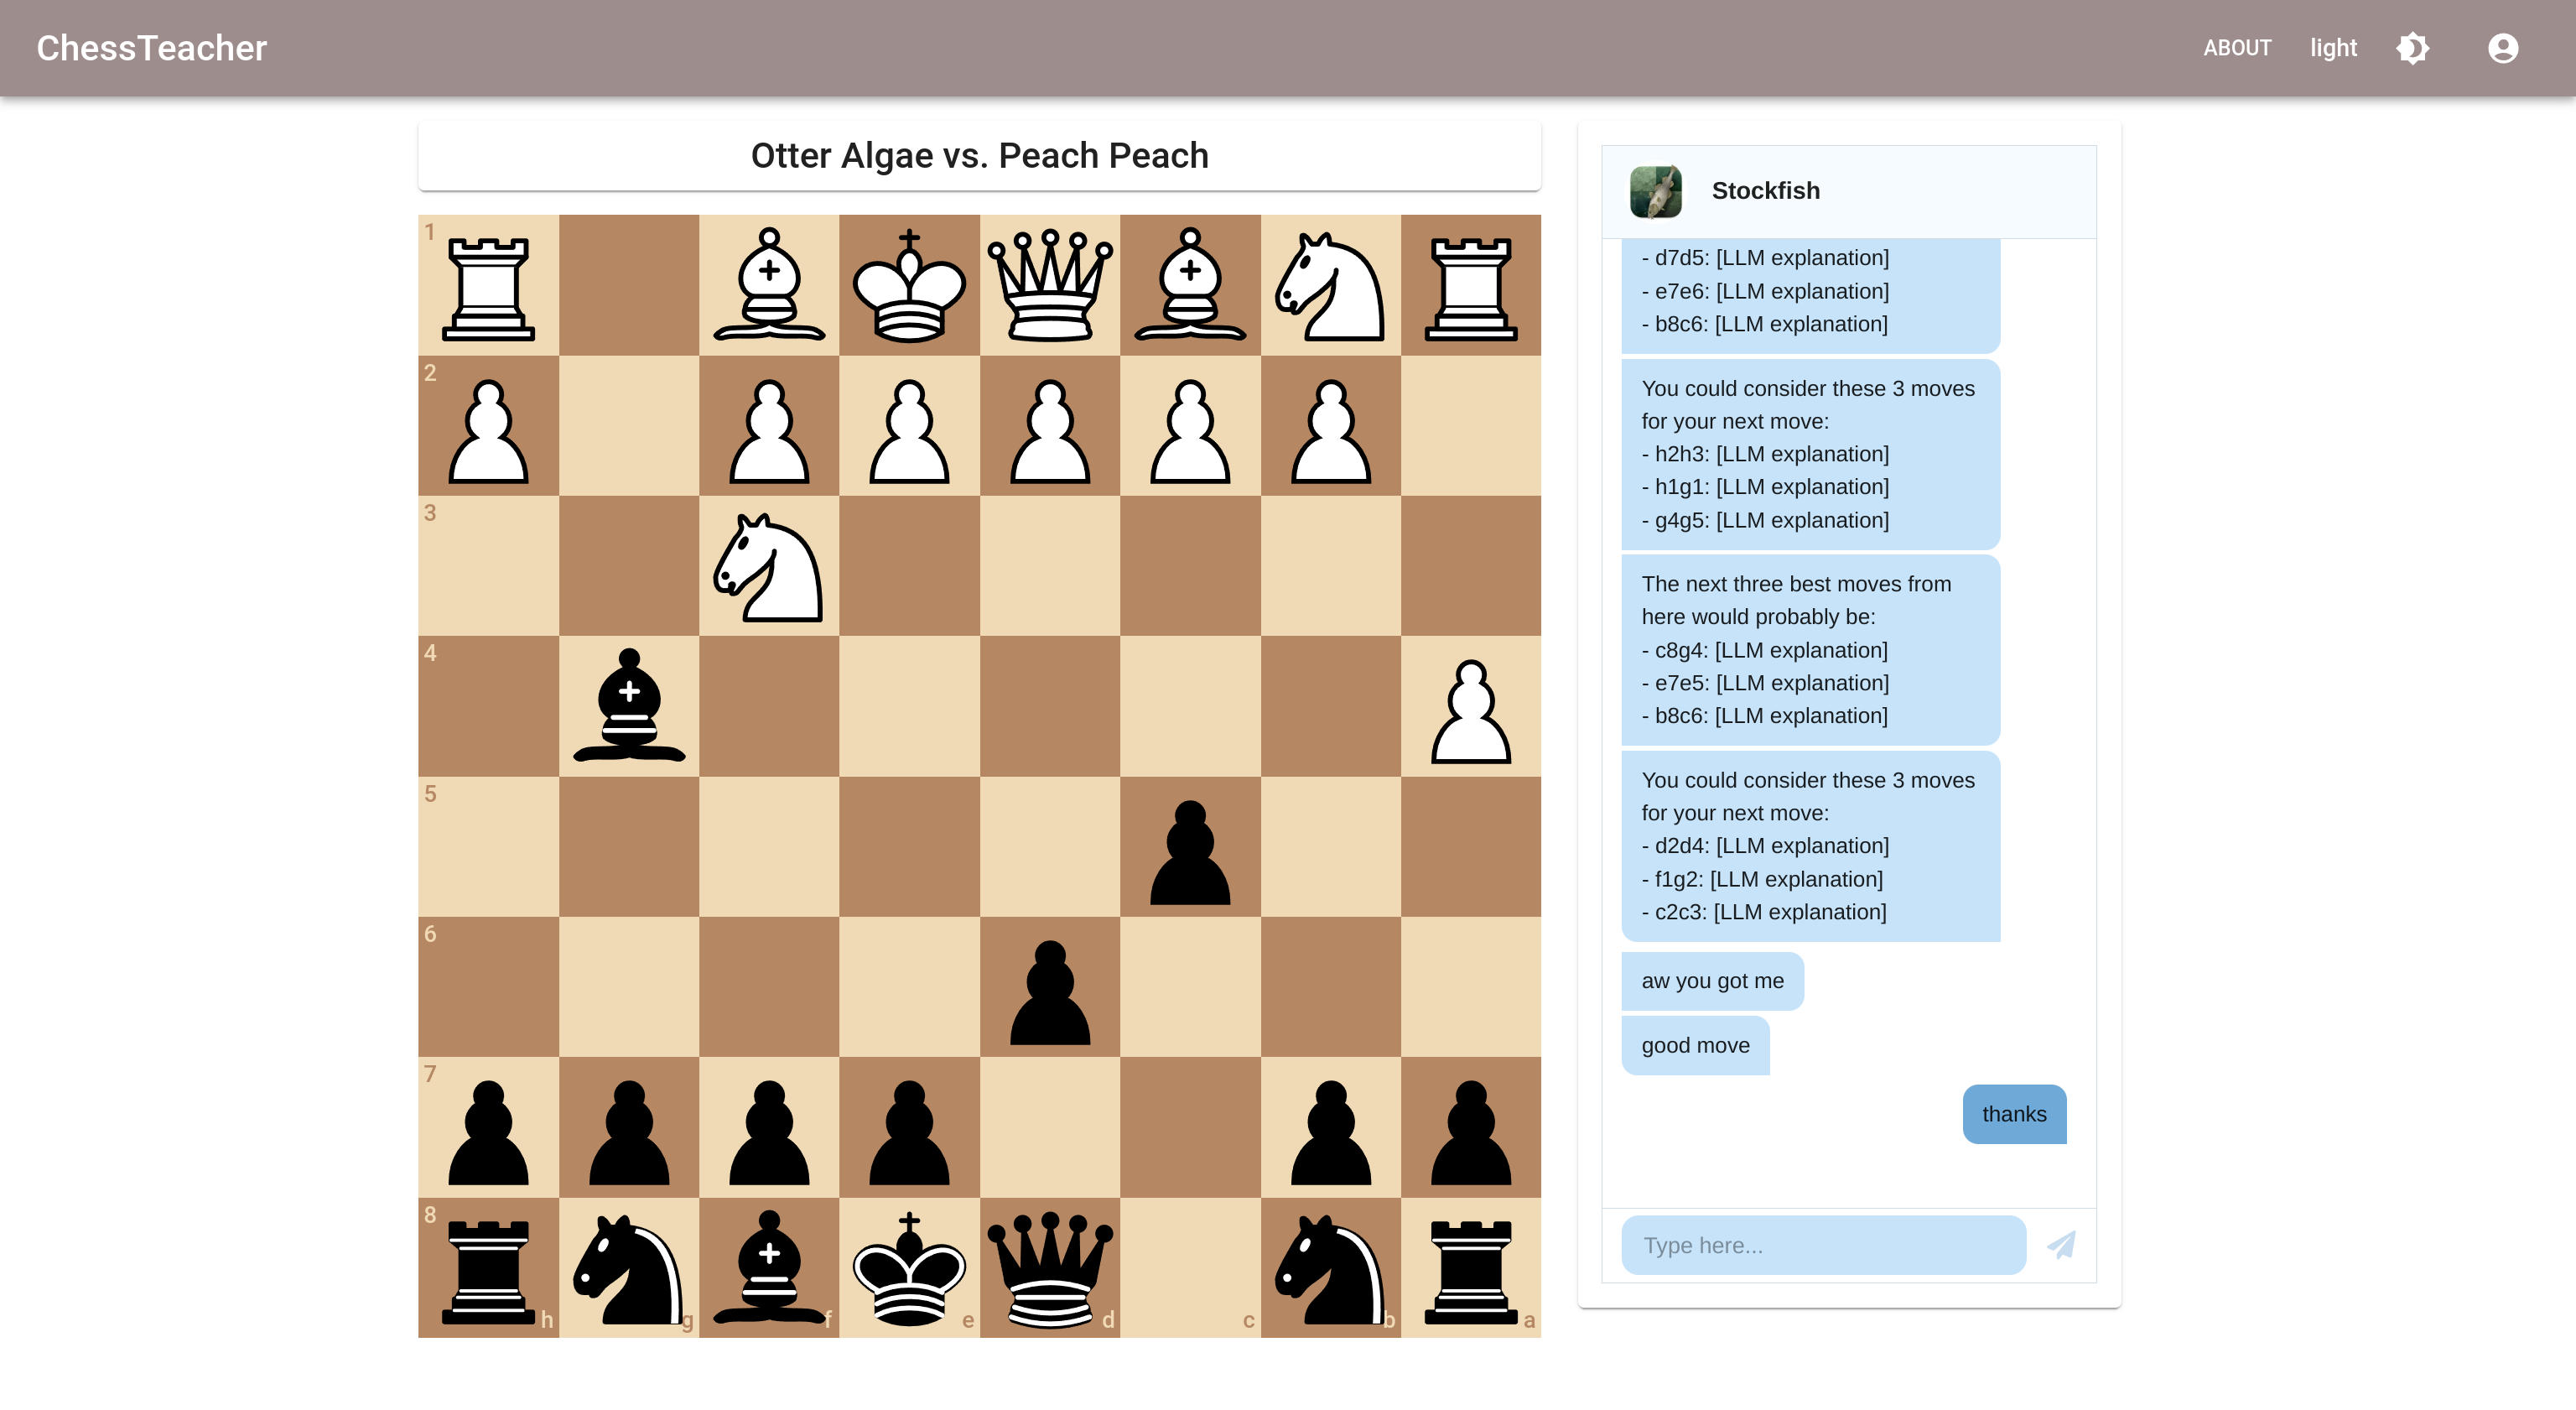
\includegraphics[width=0.85\textwidth]{Discussion-game-chat}
    \caption{What the chat could look like with an LLM.}\label{fig:Discussion-game-chat}
\end{figure}
% textidote: ignore end

The purpose of the Figure~\ref{fig:Discussion-game-chat} is
to show what it could look like if we had implemented an LLM in the project, one such as Copilot or ChatGPT\@.
The Figure~\ref{fig:llm} shows an example of a conversation with an LLM, where the user asks for an explanation
this could be implemented in the chat window in the game interface, as seen in Figure~\ref{fig:Discussion-game-chat}
instead of its placeholder text.


    % textidote: ignore begin
\section{Conclusion}\label{sec:conclusion}
% textidote: ignore end


    % Appendix
    \appendix

    % textidote: ignore begin
\chapter{Source Code Repositories}\label{ch:source-code-repositories}
% textidote: ignore end

Reference is made to our \href{https://github.com/audio-engineer/aau-p2-software}{GitHub Repository} release 1.0.0.

Link: \url{https://github.com/audio-engineer/aau-p2-software}.

    \subfile{process-analysis/process-analysis}

    % Bibliography
    \printbibliography[heading=bibintoc]
\end{document}
